\documentclass[aspectratio=169,12pt]{beamer}

\usepackage{hyperref}
\usepackage[giveninits=true,doi=false,isbn=false,url=false,eprint=false]{biblatex}



\renewbibmacro*{booktitle}{%
  \textbf{\printfield[booktitle]{booktitle}}%
}

\usepackage{subcaption}

\usepackage{amsmath}
\usepackage{bm}

\usepackage{tcolorbox}

\addbibresource{references.bib}
\addbibresource{publications_oral.bib}

\usepackage{varwidth}
\usepackage{tikz}
\usetikzlibrary{tikzmark}



\tikzset{
    blueblock/.style = {draw=amethyst,thick,fill=amethyst!15,rounded corners=0pt,inner sep=7pt}
}
\tikzset{
    pinkblock/.style = {draw=amaranth,thick,fill=amaranth!15,rounded corners=0pt,inner sep=7pt}
}

\tikzset{
    widepinkblock/.style = {draw=amaranth,thick,fill=amaranth!15,rounded corners=0pt,inner sep=20pt}
}

\usepackage{multirow}
\usepackage{booktabs}
\usepackage{algorithm}
\usepackage{algpseudocode}


\usepackage{amssymb}% http://ctan.org/pkg/amssymb
\usepackage{pifont}% http://ctan.org/pkg/pifont
\newcommand{\cmark}{\ding{51}}%
\newcommand{\xmark}{\ding{55}}%



\usepackage{xargs}

\def\param{x}
\def\varparam{y}
\def\paramlim{x_\star}
\def\rmd{\mathrm{d}}
\def\eqdef{\overset{\Delta}{=}}
\def\step{\gamma}
\def\nlupdates{H}
\def\nagent{N}
\def\Id{Id}

\def\fw{f}
\newcommandx{\nfw}[1][1=c]{f_{#1}}
\newcommandx{\nFw}[1][1=c]{F_{#1}}
\newcommandx{\nFww}[2][1=c]{\nFw[#1]^{#2}}
\newcommandx{\nf}[2][1=c]{\nfw[#1](#2)}
\newcommandx{\nfs}[3][1=c]{\nFw[#1]^{#3}(#2)}

\def\gfww{\nabla \fw}
\newcommandx{\gfw}[1]{\nabla \fw(#1)}
\newcommandx{\gnfw}[1][1=c]{\nabla \nfw[#1]}
\newcommandx{\gnf}[2][1=c]{\nabla \nfw[#1](#2)}

\newcommandx{\gnfs}[3][1=c]{\nabla \nFw[#1]^{#3}(#2)}
\newcommandx{\gnfws}[2][1=c]{\nabla \nFw[#1]^{#2}}
\newcommandx{\gfs}[3][1=c]{\nabla \fw[#1]^{#3}(#2)}

\newcommandx{\hnfw}[1][1=c]{\nabla^2 \nfw[#1]}
\newcommandx{\hnf}[2][1=c]{\nabla^2 \nfw[#1](#2)}
\newcommandx{\hf}[1]{\nabla^2 \fw(#1)}
\newcommandx{\hnfs}[3][1=c]{\nabla^2 \nFw[#1]^{#3}(#2)}

\def\hhfw{\nabla^3 \fw}
\newcommandx{\hhnfw}[1][1=c]{\nabla^3 \nfw[#1]}
\newcommandx{\hhnf}[2][1=c]{\nabla^3 \nfw[#1](#2)}
\newcommandx{\hhf}[1]{\nabla^3 \fw(#1)}


\def\covfunc{\mathcal{C}}
\newcommand{\loccovfunc}[1]{\mathcal{C}_{#1}}


\newcommand{\statdist}[1]{\pi^{(#1)}}
\newcommand{\statdistlim}[1]{\bar{x}_{\textnormal{sto}}^{(#1)}}
\newcommand{\statdistlimv}[1]{\bar{y}_{\textnormal{sto}}^{(#1)}}
\def\biasHetero{\mathrm{b}_{\mathrm{h}}}
\def\biasSto{\mathrm{b}_{\mathrm{s}}}
\newcommand{\covstatdistlim}[1]{\bar{\boldsymbol{\Sigma}}_{\textnormal{sto}}^{(#1)}}
\newcommand{\detlim}[1]{\bar{\paramw}_{\textnormal{det}}^{(#1)}}

\newcommand{\covparam}{\bar{\boldsymbol{\Sigma}}^{x}}
\newcommand{\covparamcvar}[1]{\bar{\boldsymbol{\Sigma}}^{x,\xi}_{(#1)}}
\newcommand{\covcvarparam}[1]{\bar{\boldsymbol{\Sigma}}^{\xi,x}_{(#1)}}
\newcommand{\covcvar}[1]{\bar{\boldsymbol{\Sigma}}^{\xi}_{(#1)}}
\newcommand{\covonestep}{\bar{\boldsymbol{\Sigma}}^{\epsilon}}


\definecolor{darkspringgreen}{rgb}{0.09, 0.45, 0.27}
\definecolor{amaranth}{rgb}{0.9, 0.17, 0.31}
\definecolor{amethyst}{rgb}{0.6, 0.4, 0.95}

\usepackage{enumitem}

% Labels for items in (nested) itemize (uses bullets/characters)
\newcommand\labelitemi{\textcolor{amaranth}{\textbullet}}% bullet
\newcommand\labelitemii{\textcolor{amaranth}{\normalsize\normalfont\bfseries \textendash}}% --
\newcommand\labelitemiii{\textcolor{amaranth}{\textasteriskcentered}}% *
\newcommand\labelitemiv{\textcolor{amaranth}{\textperiodcentered}}% .
\setlist[enumerate,1]{label={\textcolor{amaranth}{\arabic*.}}}


% footnote size
\makeatletter
\newcommand\notsotiny{\@setfontsize\notsotiny\@vipt\@viipt}
\makeatother

\setbeamerfont{footnote}{size=\notsotiny}


\makeatletter
\newcommand{\Pause}[1][]{\unless\ifmeasuring@\relax
\pause[#1]%
\fi}
\makeatother
%%%%%% Template things

% space between paragraphs
\parskip=1em

% title font
\setbeamerfont{title}{size=\LARGE}%, series=\bfseries}
\setbeamerfont{frametitle}{size=\LARGE}%, series=\bfseries}
\setbeamerfont{institute}{size=\normalsize}%, series=\bfseries}

% spacing between frame title and content
\addtobeamertemplate{frametitle}{\vspace*{0.2cm}}{\vspace*{0.5cm}\setcounter{footnote}{0}}

% color
\definecolor{beamer@blendedblue}{rgb}{0.8, 0, 0.34}%{0.44, 0.16, 0.39}

% no navigation
\beamertemplatenavigationsymbolsempty

% slide numbers
\setbeamertemplate{footline}
{
  \hbox{\begin{beamercolorbox}[wd=1\paperwidth,ht=5.25ex,dp=4ex,right]{framenumber}%
      \large \insertframenumber{}~~
    \end{beamercolorbox}}%
  \vskip0pt%
}

% slide numbers
\def\setupappendix{
\setcounter{framenumber}{0}
\setbeamertemplate{footline}
{
  \hbox{\begin{beamercolorbox}[wd=1\paperwidth,ht=5.25ex,dp=4ex,right]{framenumber}%
      \large A-\insertframenumber{}~~
    \end{beamercolorbox}}%
  \vskip0pt%
}
}


% centered titles
\makeatletter
\long\def\beamer@@frametitle[#1]#2{%
  \beamer@ifempty{#2}{}{%
    \gdef\insertframetitle{\centering{#2\ifnum\beamer@autobreakcount>0\relax{}\space\usebeamertemplate*{frametitle continuation}\fi}}%
  \gdef\beamer@frametitle{#2}%
  \gdef\beamer@shortframetitle{#1}%
}%
}
\makeatother

%%%%% Equations

\newcounter{mytn}
\makeatletter
\newcommand{\tmn}[3][]{\stepcounter{mytn}%
\tikzmarknode[Col\the\numexpr\value{mytn}-\mytn@start\relax/.try,inner xsep=2pt,%
minimum height=1.6em,inner sep=2mm,#1]{mytn-\number\value{mytn}}{#2}%
\expandafter\gdef\csname tmn@annot@\number\value{mytn}\endcsname{#3}}
\newenvironment{AnnotatedEquation}{\edef\mytn@start{\number\value{mytn}}%
\begin{equation*}}{\end{equation*}%
\edef\mytn@end{\number\value{mytn}}%
\ifnum\mytn@end>\mytn@start
\begin{itemize}
 \foreach \X in {\the\numexpr\mytn@start+1,...,\mytn@end}
 {\item \tikzmarknode{mytn-annot-\X}{\csname tmn@annot@\X\endcsname}%
   \begin{tikzpicture}[overlay,remember picture]
  \draw[-stealth] (mytn-annot-\X.east) to[out=0,in=-90] (mytn-\X.south);
 \end{tikzpicture}}
\end{itemize}
\fi}
\makeatother
\tikzset{ Col1/.style= {fill=blue!20,anchor=base,rounded corners=2pt},
Col2/.style= {Col1, fill=red!20},
Col3/.style= {Col1, fill=green!20},
Col4/.style= {Col1, fill=yellow!20},
}

% footnotes at end of frame rather than minipage

\makeatletter
\renewrobustcmd{\blx@mkbibfootnote}[2]{%
  \iftoggle{blx@footnote}
    {\blx@warning{Nested notes}%
     \addspace\mkbibparens{#2}}
    {\unspace
     \ifnum\blx@notetype=\tw@
       \expandafter\@firstoftwo
     \else
       \expandafter\@secondoftwo
     \fi
       {\csuse{blx@theendnote#1}{\protecting{\blxmkbibnote{end}{#2}}}}
       {\csuse{footnote}[frame]{\protecting{\blxmkbibnote{foot}{#2}}}}}}
\makeatother

%%%%% INFORMATION

\title{\LARGE Convergence and Linear Speed-Up in Stochastic Federated Learning  \\[0.5em]
\normalsize (or: Taming Heterogeneity in Federated Linear Stochastic Approximation)
\vspace{0em}}
\author{
  Paul Mangold (CMAP, École polytechnique) \\[0.5em]
  ICCOPT 2025 --  Federated optimization and learning algorithms
}
\titlegraphic{
}
\institute{}
\date{July 23rd, 2025}


%%%%% DOCUMENT

\begin{document}

%% TITLE PAGE

\begin{frame}[plain]
  \vspace{3.5em}
  \titlepage
\end{frame}
\addtocounter{framenumber}{-1}



\begin{frame}[t]{Federated Learning}
% \footfullcite{mangold2020decentralized}$^{,}$\footfullcite{ogier2022flamby}$^{,}$\footfullcite{mangold2024scafflsa}$^{,}$\footfullcite{mangold2025refined}$^{,}$\footfullcite{mangold2025scaffold}}
\vspace{0.5em}
  \begin{minipage}{0.35\linewidth}
    \begin{center}
    % 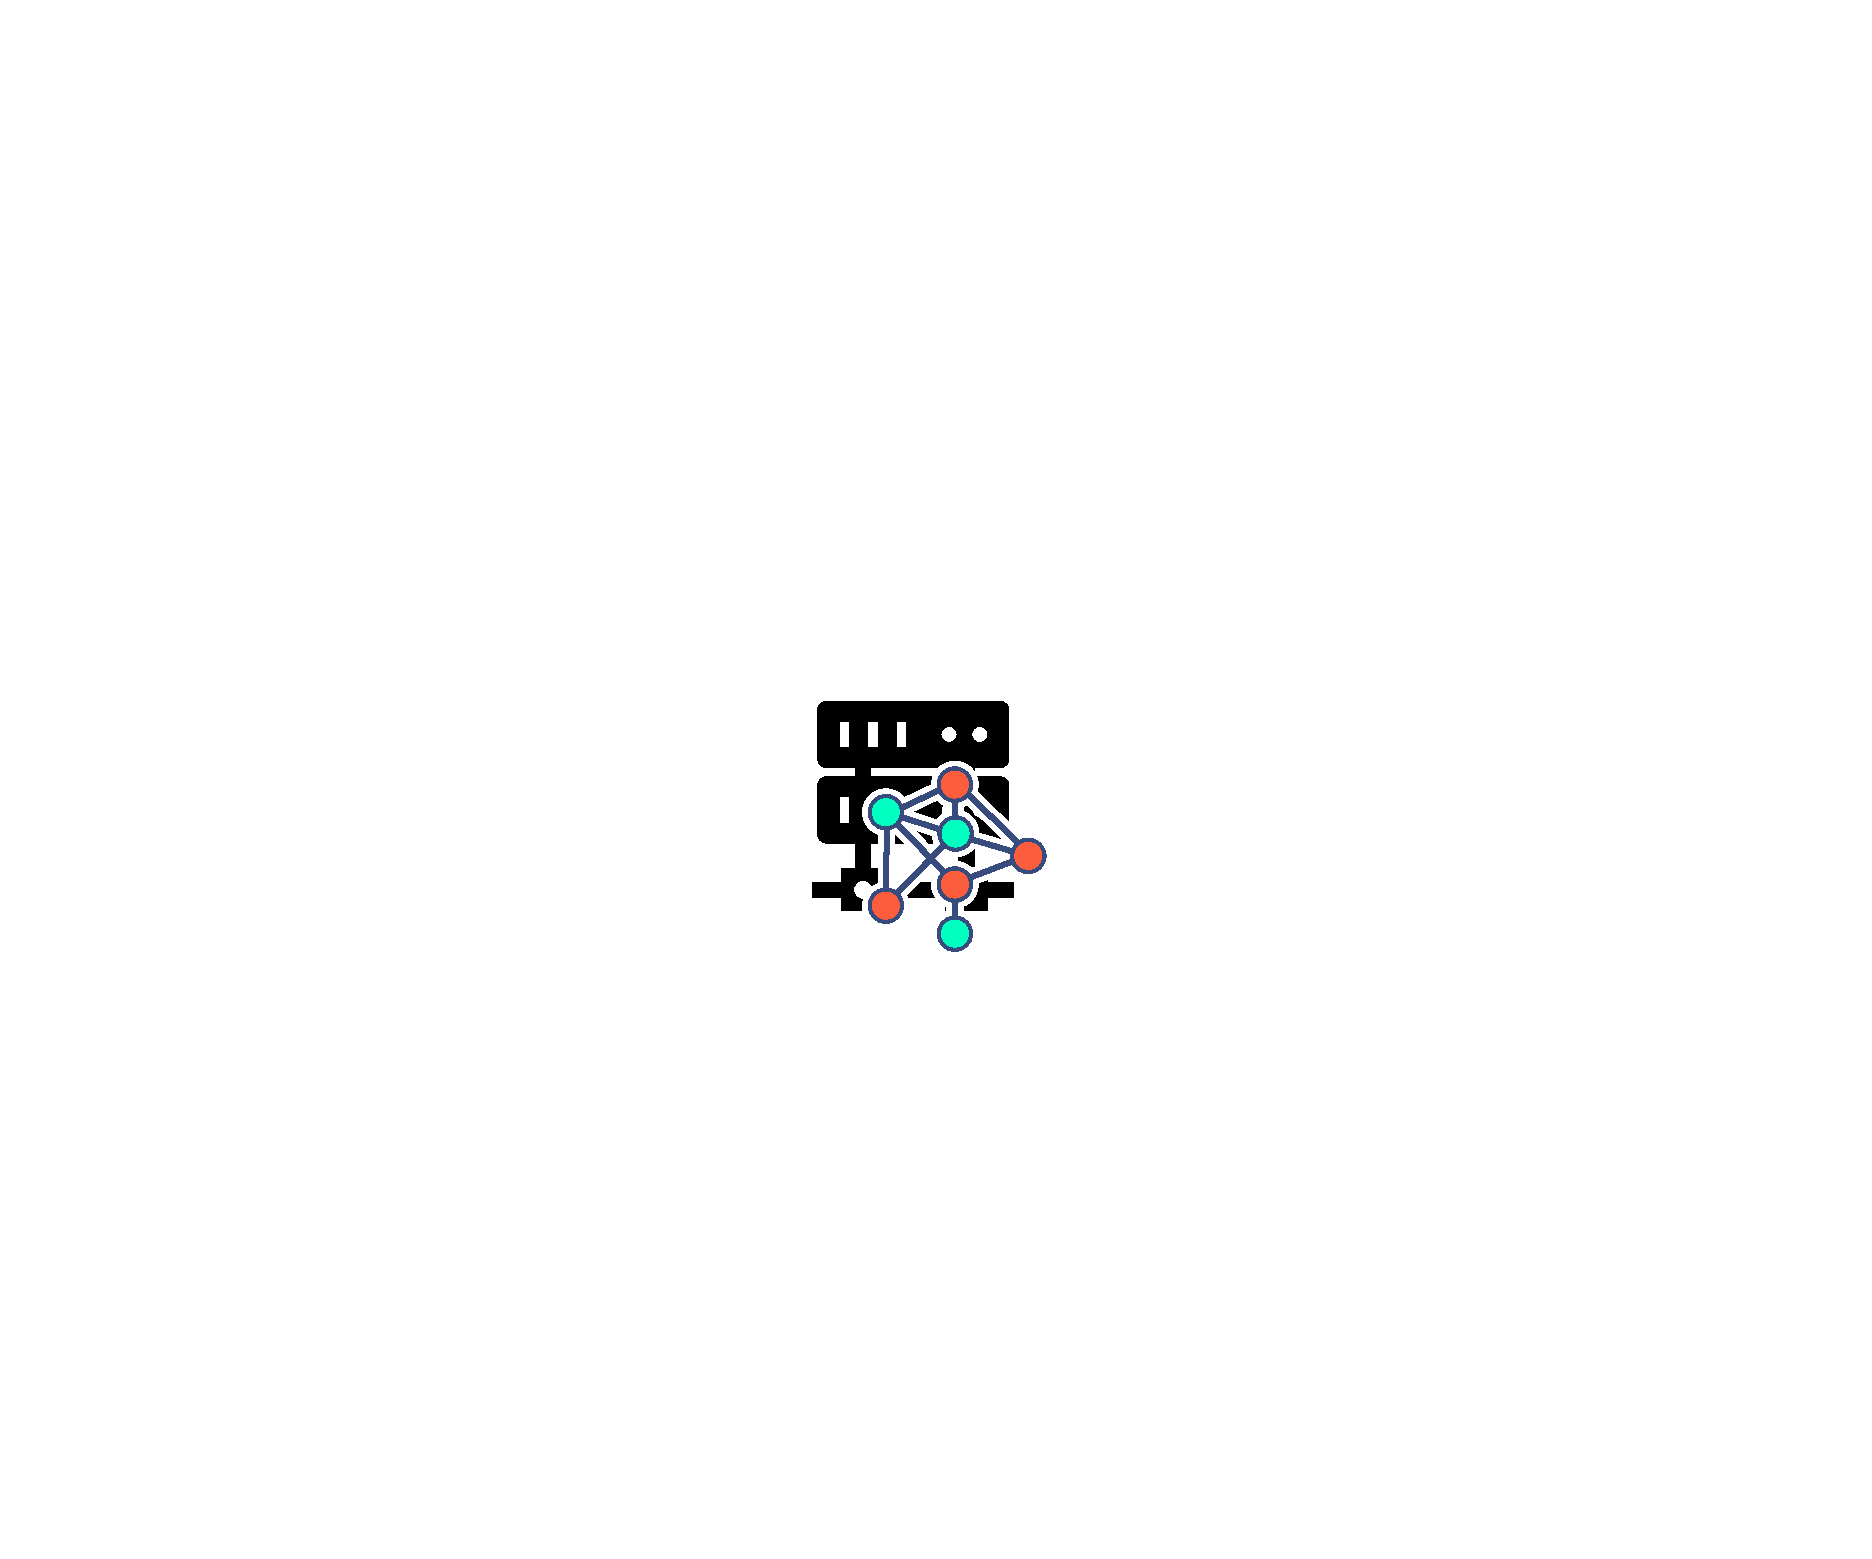
\includegraphics[width=\linewidth]{images/federated_learning_only_server.pdf} }%
    % \only<2,3,4>{    
    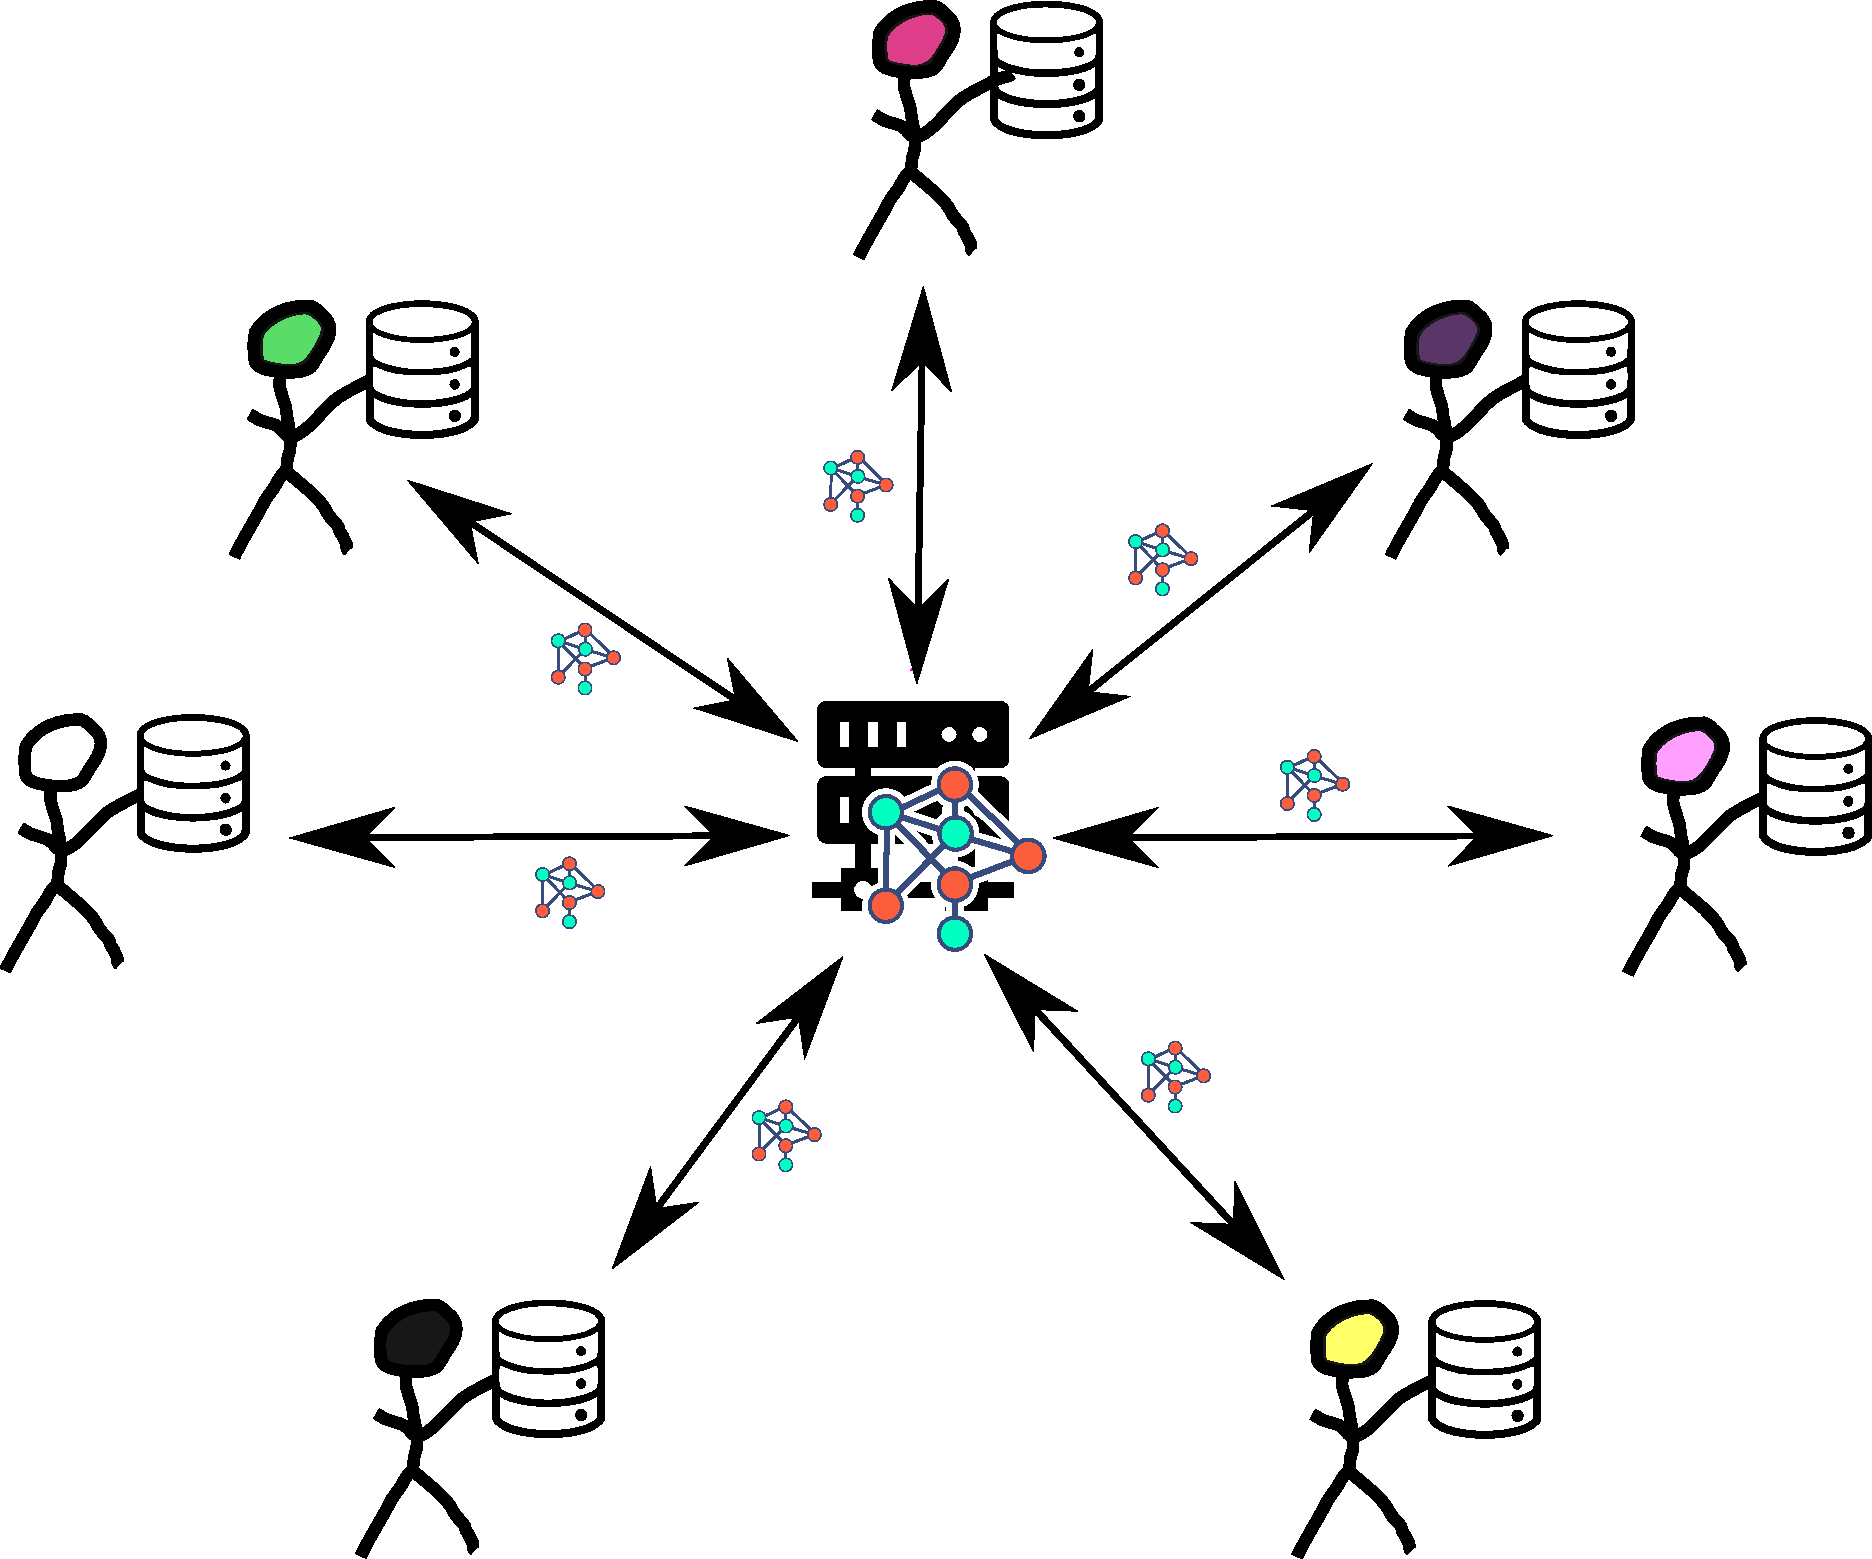
\includegraphics[width=\linewidth]{images/federated_learning.pdf} 
    % }
    \end{center}
    
  \end{minipage}~~~~~~%
  \begin{minipage}{0.5\linewidth}

%\only<3,4>{
    \begin{center}
      Collaborative optimization problem
      \begin{align*}
        \min_{x \in \mathbb{R}^d} 
        \frac{1}{N} \sum_{c=1}^N f_c(x)
        ~~,
        \quad 
        f_c(x)
        = \mathbb{E}_{Z \sim D_c} [ F_c(x; Z) ]
      \end{align*}
      % $\rightarrow$ avec une seule \emph{solution globale}
    \end{center}
 %   }
      
  \end{minipage}

% \vspace{0.5em}

% \only<4>{
%   \begin{center}
%       \textbf{\textcolor{purple}{Difficultés centrales}} : hétérogénéité des données et des moyens de calcul 

%       \vspace{-0.5em}
      
%       + communication lente et difficile à établir
%   \end{center}
% }
  \begin{center}
      \textbf{\textcolor{purple}{Central Challenges}}: data and computational heterogeneity 

      \vspace{-0.5em}
      
      + slow and difficult-to-establish communication
  \end{center}
\end{frame}
% \begin{frame}[t]{Federated Learning}
% % \footfullcite{mangold2020decentralized}$^{,}$\footfullcite{ogier2022flamby}$^{,}$\footfullcite{mangold2024scafflsa}$^{,}$\footfullcite{mangold2025refined}$^{,}$\footfullcite{mangold2025scaffold}}
% \vspace{0.5em}
%   \begin{minipage}{0.35\linewidth}
%     \begin{center}
%     \only<1>{    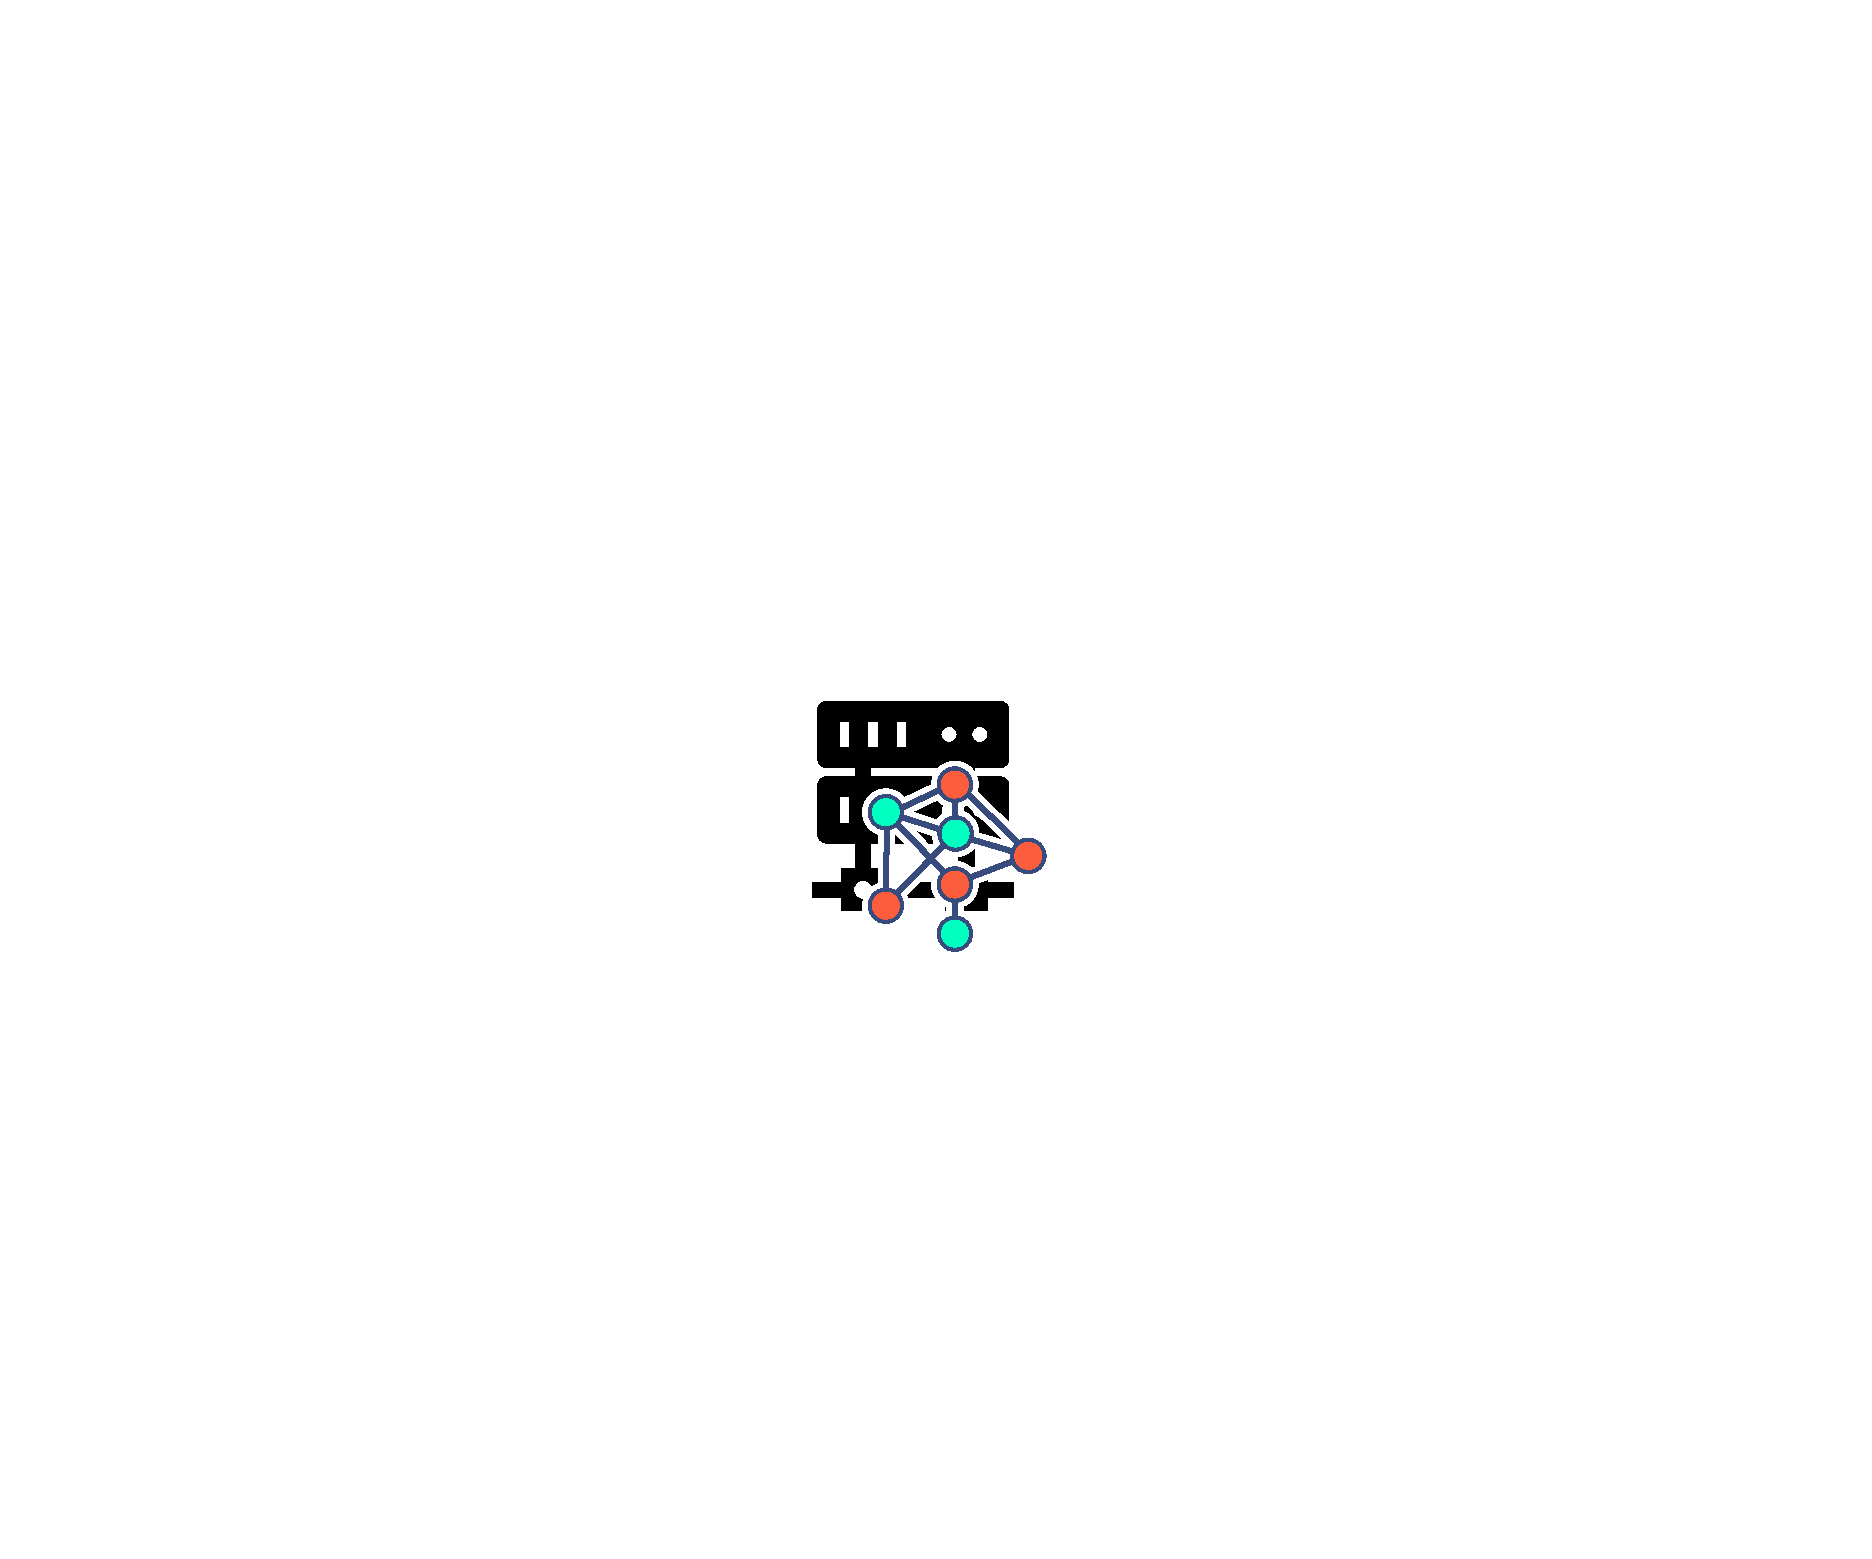
\includegraphics[width=\linewidth]{images/federated_learning_only_server.pdf} }%
%     \only<2,3,4>{    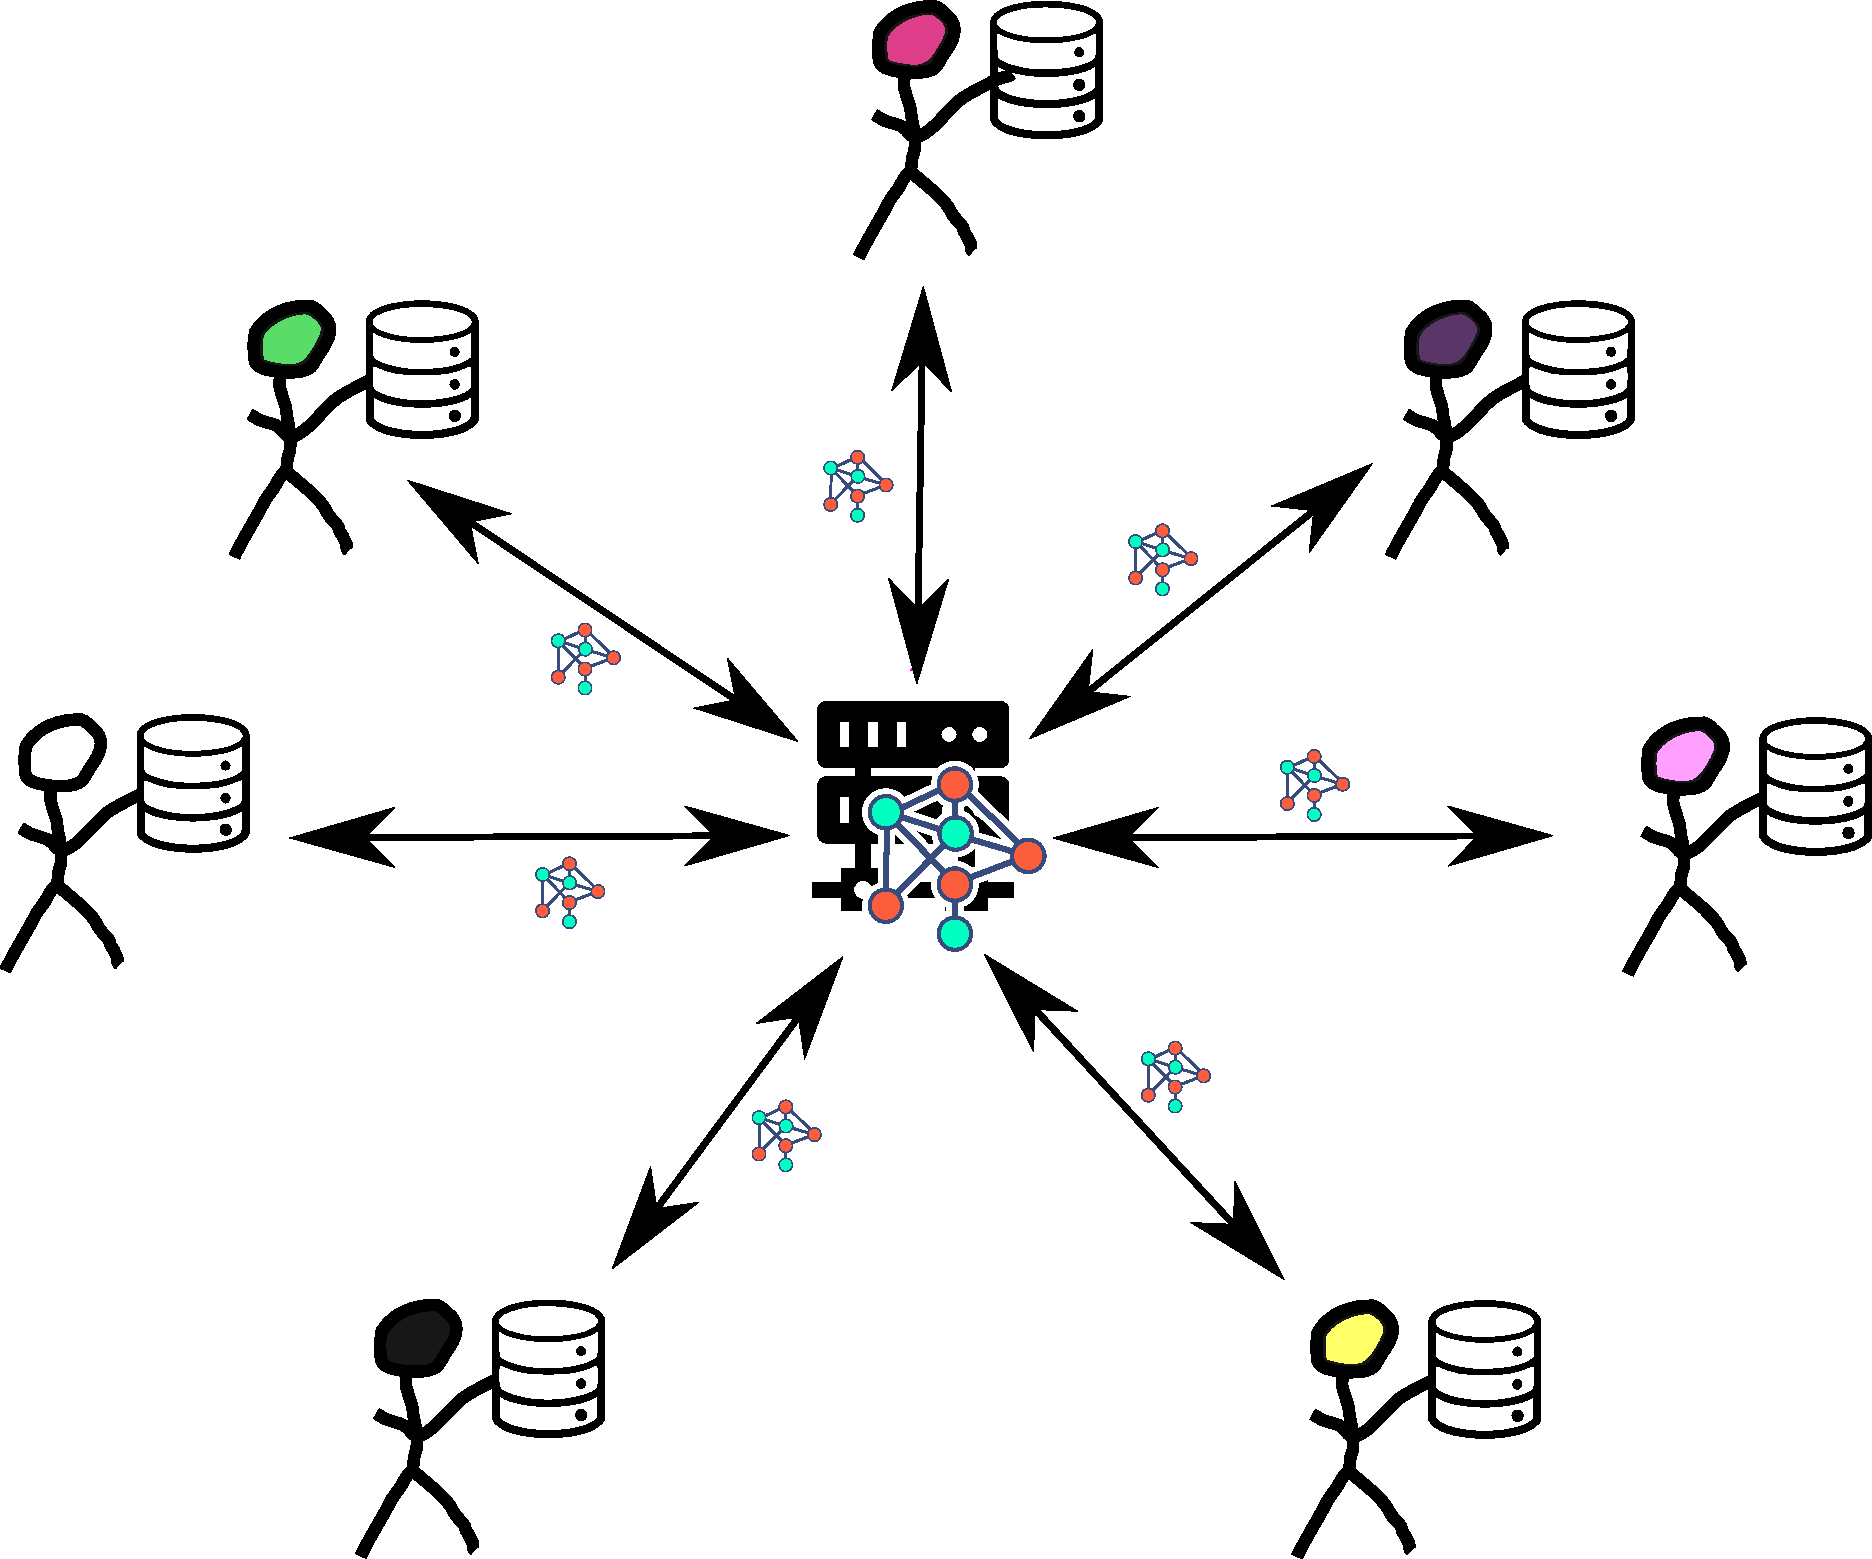
\includegraphics[width=\linewidth]{images/federated_learning.pdf} }
%     \end{center}
    
%   \end{minipage}~~~~~~%
%   \begin{minipage}{0.5\linewidth}

% \only<3,4>{
%     \begin{center}
%       Collaborative optimization problem
%       \begin{align*}
%         \min_{x \in \mathbb{R}^d} 
%         \frac{1}{N} \sum_{c=1}^N f_c(x)
%         ~~,
%         \quad 
%         f_c(x)
%         = \mathbb{E}_Z[ F_c(x; Z) ]
%       \end{align*}
%       % $\rightarrow$ avec une seule \emph{solution globale}
%     \end{center}
%     }
      
%   \end{minipage}

% % \vspace{0.5em}

% % \only<4>{
% %   \begin{center}
% %       \textbf{\textcolor{purple}{Difficultés centrales}} : hétérogénéité des données et des moyens de calcul 

% %       \vspace{-0.5em}
      
% %       + communication lente et difficile à établir
% %   \end{center}
% % }
%   \pause
%   \pause
%   \pause
%   \begin{center}
%     \textcolor{purple}{\bfseries Problem: data is heterogeneous, communication is expensive}
%   \end{center}
  
% \end{frame}




\begin{frame}
  \begin{center}
    \huge \textcolor{purple}{
      I. Federated Averaging
      }
  \end{center}
\end{frame}



\begin{frame}[t]{Federated Averaging\footfullcite{mcmahan2017communicationoral} ~~~ \raisebox{0.2em}{\textcolor{black}{\normalsize $x^\star \in \arg\min_{x \in \mathbb{R}^d} 
    \frac{1}{N} \sum_{c=1}^N \mathbb{E}_Z[ F_c(x; Z) ]$}} ~~}  
    
    \vspace{1em}

  \begin{minipage}{0.5\linewidth}

  \footnotesize
  At each global iteration

    \begin{itemize}[leftmargin=*,itemsep=0em]
  \footnotesize
    \item For $c=1$ à $N$ in parallel

\vspace{-0.2em}
    
    
\begin{itemize}[leftmargin=*,itemsep=0em]
\item Receive $x^{(t)}$, set $x^{(t,0)}_c = x^{(t)}$
    
        \item For $h=0$ to $H-1$
    \end{itemize}

\vspace{-0.6em}
\begin{center}
            \hspace{-1em}$x^{(t,h+1)}_c = x^{(t,h)}_c - \gamma \nabla F_c( x^{(t,h)}_c ; Z_c^{(t,h+1)})$
        \end{center}
      
  \item Aggregate local models 
        
        
\vspace{-0.6em}
\begin{center}
            \hspace{-1em}$x^{(t+1)} = \frac{1}{N} \sum_{c=1}^N x_c^{(t,H)}$
        \end{center}
      
    \end{itemize}
      
  \end{minipage}~%
  \begin{minipage}{0.48\linewidth}
    \pause
    \begin{center}
      \small
    With deterministic gradients:
    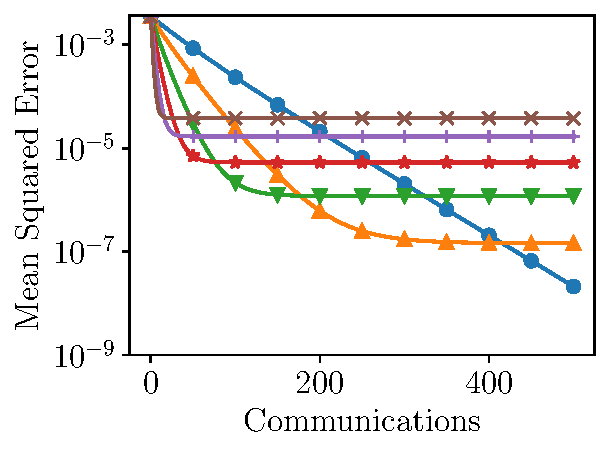
\includegraphics[width=0.75\linewidth]{images/local_training_heterogeneous.pdf}%
    \raisebox{2.5em}{ 
\includegraphics[width=0.25\linewidth]{images/legend.pdf} }
  \end{center}
  
  %   \vspace{-0.5em}

  % ~~~~Plus d'itérations locales

  %   \vspace{0.5em}
    
  %   ~~~~~{\large \textcolor{green} \cmark}\, convergence plus rapide
    
  %   ~~~~~{\large \textcolor{red} \xmark}~ biais plus grand

  \end{minipage}

  \vspace{1.5em}


\end{frame}

\begin{frame}{Classical analyses of this algorithm\\[-0.5em]
    \small (For $L$-smooth, $\mu$-strongly convex functions)}

  Choose your favorite heterogeneity measure
  \pause
  \begin{itemize}
  \item first-order\footfullcite{lian2017can}: $\zeta = \frac{1}{N} \sum_{c=1}^N \big\| \nabla f_c(x^{\star}) - \nabla f(x^{\star}) \big\|^2$
  
  \pause
  
  \item second-order\footfullcite{khaled2022faster}: $\zeta = \frac{1}{N} \sum_{c=1}^N \big\| \nabla_c^2 f(x^{\star}) - \nabla^2 f(x^{\star}) \big\|^2$
  
  \pause
  
  \item average drift\footfullcite{wang2024Unreasonable}: $\zeta = \big\| \frac{1}{NH} \sum_{c=1}^N \sum_{h=0}^{H-1} \nabla f(x_c^{(h)}) - \nabla f(x^{\star}) \big\|^2$
  \end{itemize}

  %\vspace{0.5em}

  \pause

  Show \textcolor{purple}{\bfseries convergence to a neighborhood} of $x^\star$
  \begin{align*}
    \| x^{(T)} - x^\star \|^2 \lesssim (1 - \gamma \mu)^{HT} \| x^{(0)} - x^\star \|^2
    + \textcolor{purple}{\boldsymbol{\chi(\gamma, H, \zeta)}} ~~~~~\text{\small (for some function $\chi$)}
  \end{align*}

  \vspace{1em}

  
\end{frame}


\begin{frame}[t]
  \vspace{-1em} 
\begin{align*}
    \| x^{(T)} - x^\star \|^2 \lesssim (1 - \gamma \mu)^{HT} \| x^{(0)} - x^\star \|^2
    + \textcolor{purple}{\boldsymbol{\chi(\gamma, H, \zeta)}} ~~~~~\text{\small (for some function $\chi$)}
  \end{align*}
  \vspace{-2em} 
  \begin{center}
    
  \resizebox{0.9\linewidth}{!}{
  \begin{tikzpicture}
    \draw [-to,very thick](0,0) -- (12.5,0);
    \node at (1.5,0.2) {$H=2$};
    \node at (6,0.2) {$H=10$};
    \node at (10.5,0.2) {$H=50$};
  \end{tikzpicture}
}
\vspace{-0.5em}

\only<1>{
  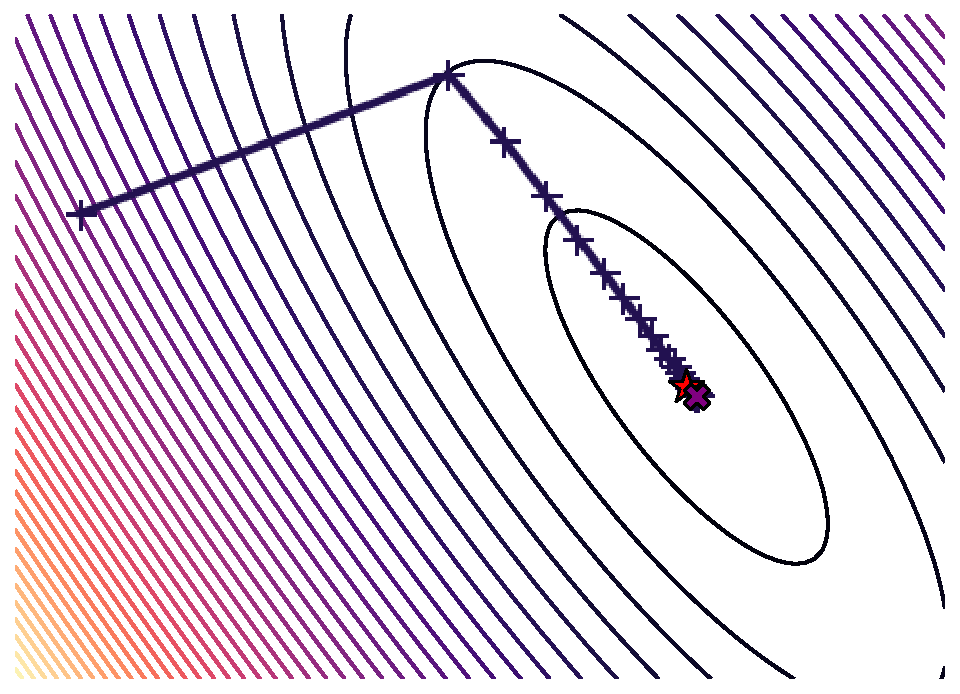
\includegraphics[width=0.3\linewidth]{images/plots/fedavg_False_2_t1000_s0.pdf}
  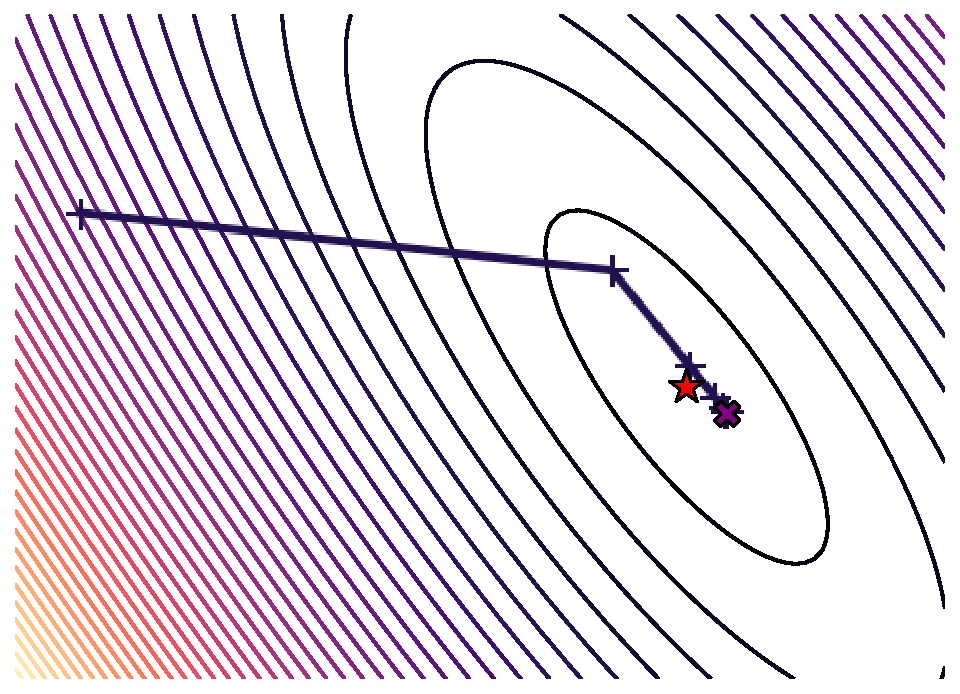
\includegraphics[width=0.3\linewidth]{images/plots/fedavg_False_10_t1000_s0.pdf}
  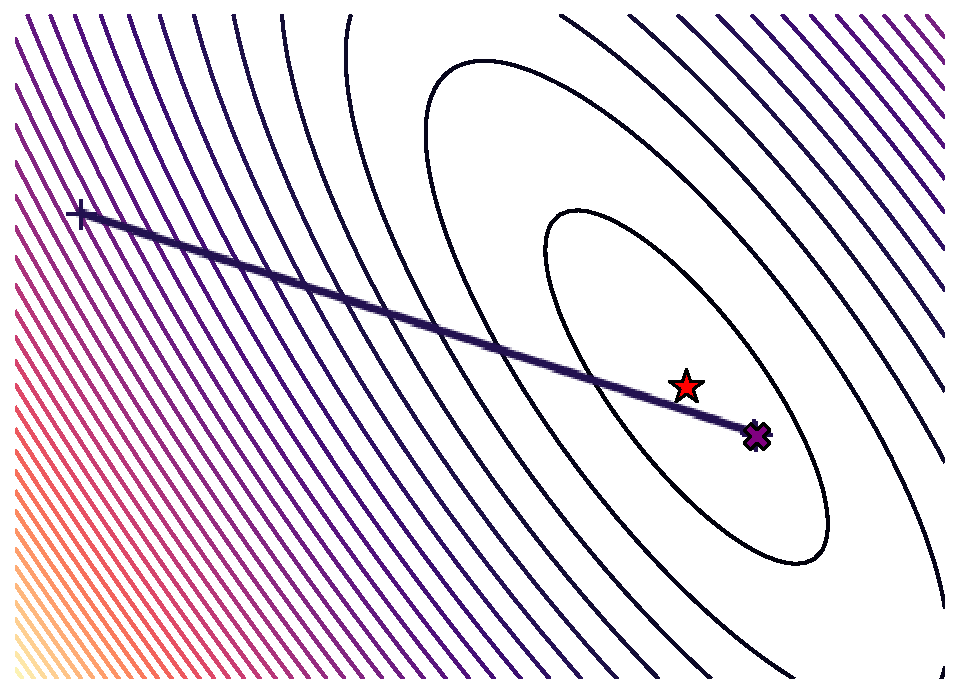
\includegraphics[width=0.3\linewidth]{images/plots/fedavg_False_50_t1000_s0.pdf}
}%
\only<2>{
  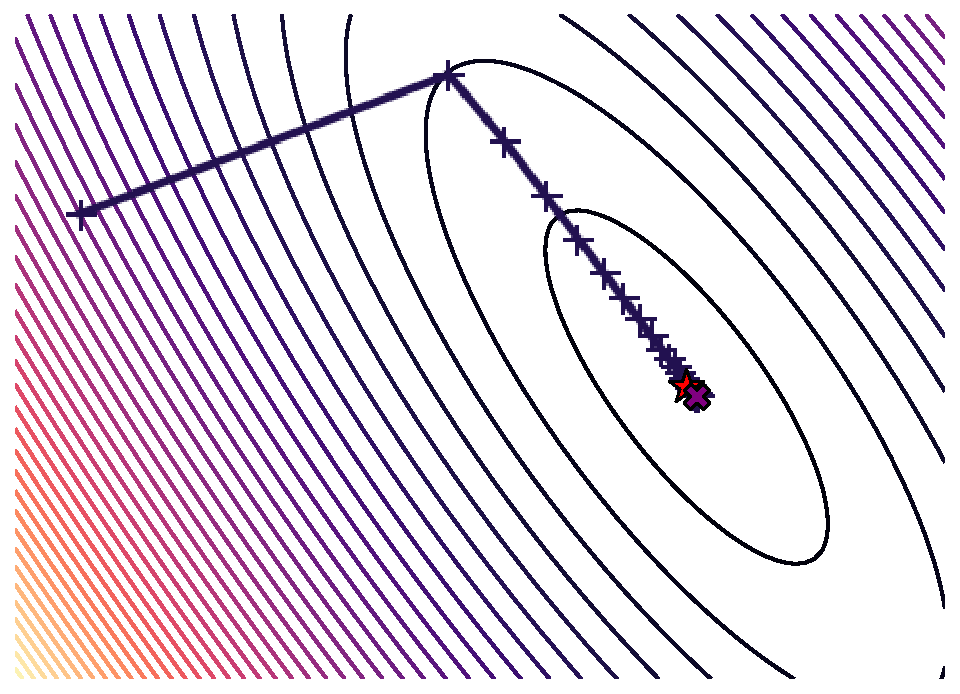
\includegraphics[width=0.3\linewidth]{images/plots/fedavg_True_2_t1000_s0.pdf}
  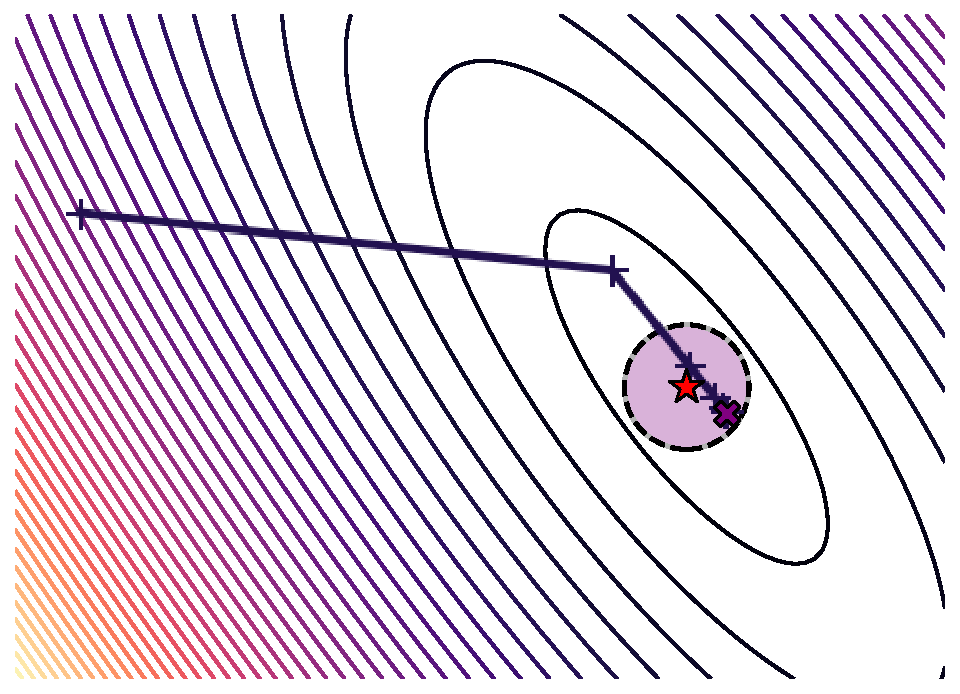
\includegraphics[width=0.3\linewidth]{images/plots/fedavg_True_10_t1000_s0.pdf}
  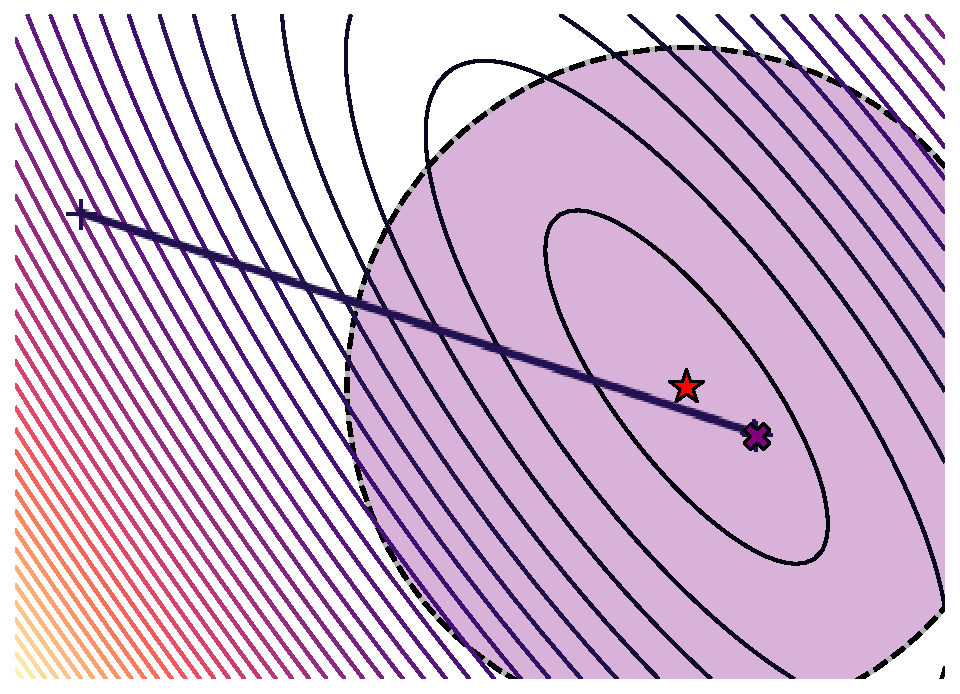
\includegraphics[width=0.3\linewidth]{images/plots/fedavg_True_50_t1000_s0.pdf}
}%
% \only<4>{
%   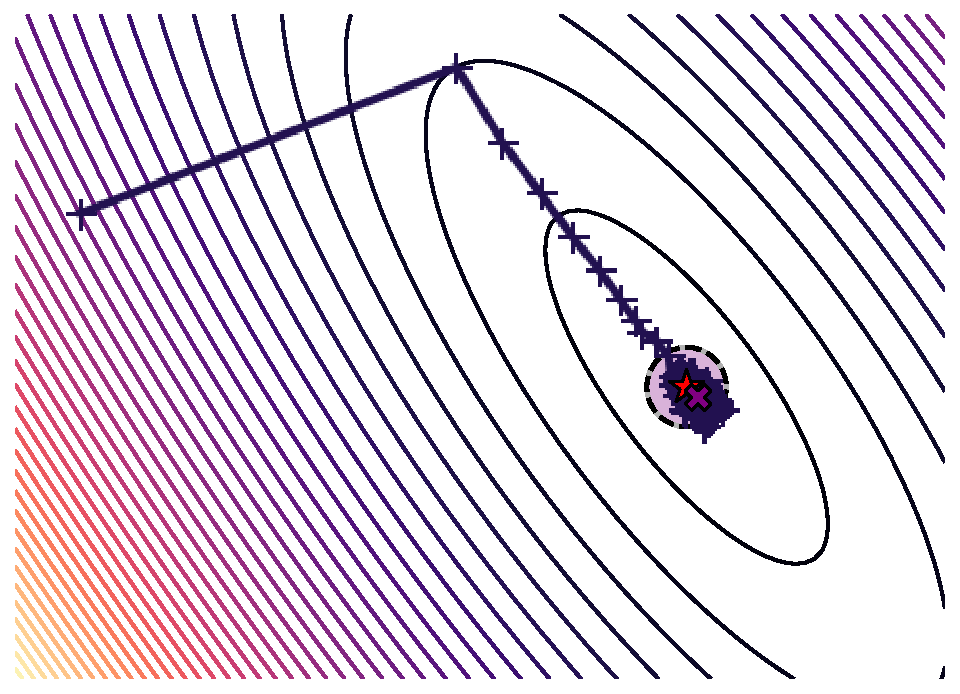
\includegraphics[width=0.3\linewidth]{images/plots/fedavg_True_2_t1000_s1.pdf}
%   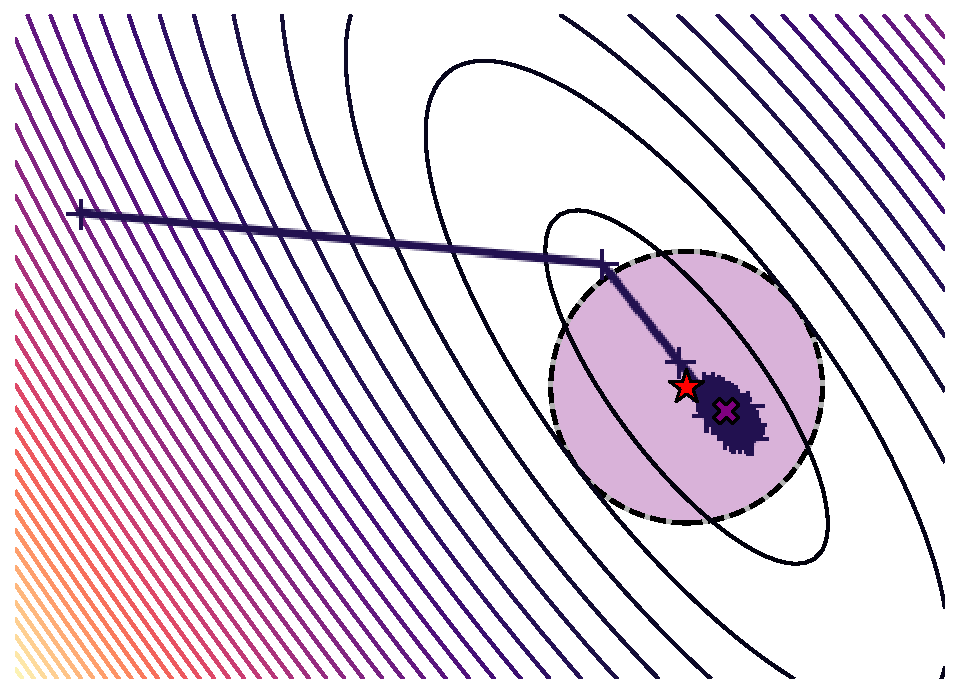
\includegraphics[width=0.3\linewidth]{images/plots/fedavg_True_10_t1000_s1.pdf}
%   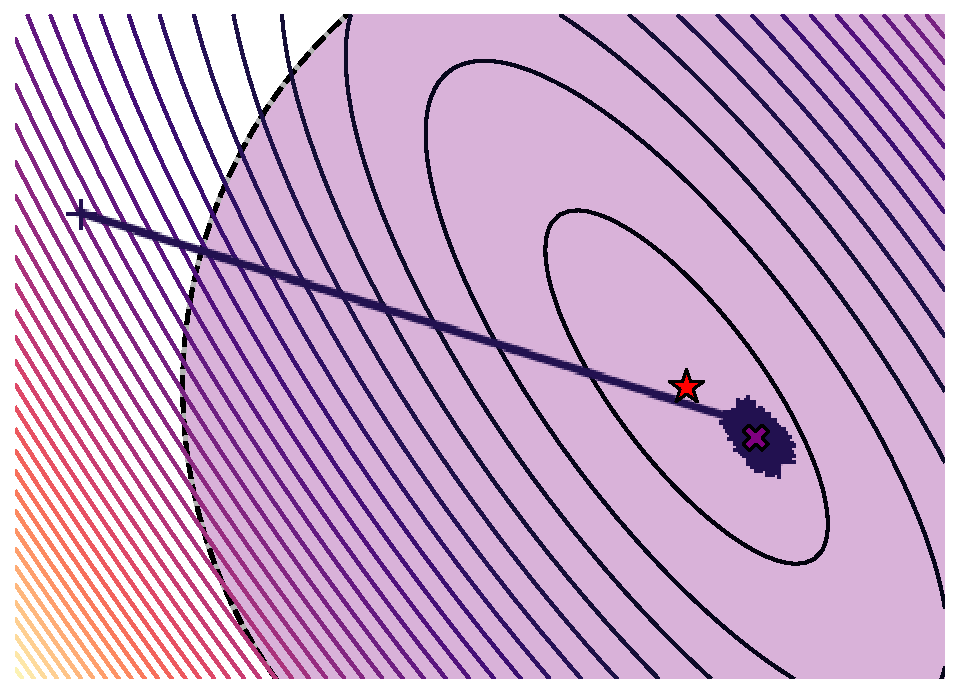
\includegraphics[width=0.3\linewidth]{images/plots/fedavg_True_50_t1000_s1.pdf}
% }

\vspace{-3em}

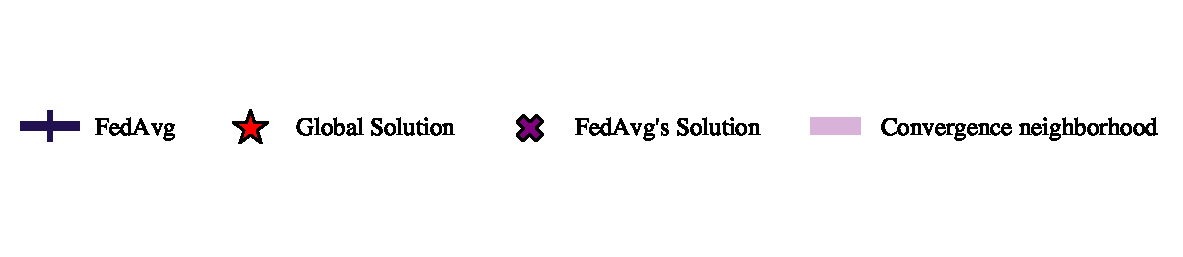
\includegraphics[width=0.8\linewidth]{images/legend_fedavg.pdf}    
    
  \end{center}

  \vspace{-3em}

  \begin{center}
    When the number of local iterations increases, bias incrases
    
  \vspace{-0.5em}

    \pause
    
  %   ... but the bound is oblivious to problem's geometry
    

  % \pause

  \vspace{-0.5em}
  
  \textcolor{purple}{\bfseries Remark:} It seems that iterates converge in some way?
  \end{center}
  
\end{frame}

\begin{frame}{Federated Averaging as Fixed Point Iteration}

    Remark that, starting with $x_c^{(t)}, y_c^{(t)} \in \mathbb{R}^d$,
    \begin{align*}
        x_c^{(t,h+1)} - 
        y_c^{(t,h+1)}
        =
        x_c^{(t,h)} -
        y_c^{(t,h)}
        - \gamma ( \nabla f_c( x_c^{(t,h)} ) - \nabla f_c(y_c^{(t,h)}) )
    \end{align*}

    Thus
    \begin{align*}
    \| x_c^{(t+1)} - y_c^{(t+1)} \|
    \le
    (1 - \gamma \mu)^H \| x_c^{(t)} - y_c^{(t)} \|
    \end{align*}

    \pause

\begin{center}
\large 
    \textcolor{purple}{$\Rightarrow$ deterministic FedAvg converges to a unique point\footfullcite{malinovskiy2020local}} 
\end{center}
\end{frame}

\begin{frame}[t]{Open Question: What about the Stochastic Case?}
  \vspace{-1em} 
  \pause

  \begin{center}
    
  \resizebox{0.9\linewidth}{!}{
  \begin{tikzpicture}
    \draw [-to,very thick](0,0) -- (12.5,0);
    \node at (1.5,0.2) {$H=2$};
    \node at (6,0.2) {$H=10$};
    \node at (10.5,0.2) {$H=50$};
  \end{tikzpicture}
}
\vspace{-0.5em}

  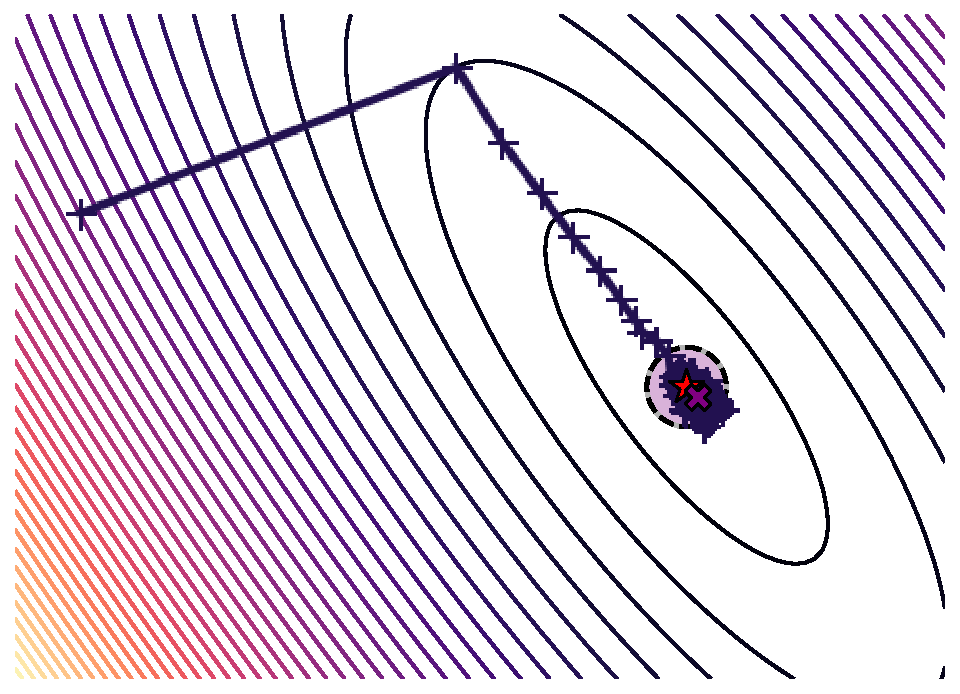
\includegraphics[width=0.3\linewidth]{images/plots/fedavg_True_2_t1000_s1.pdf}
  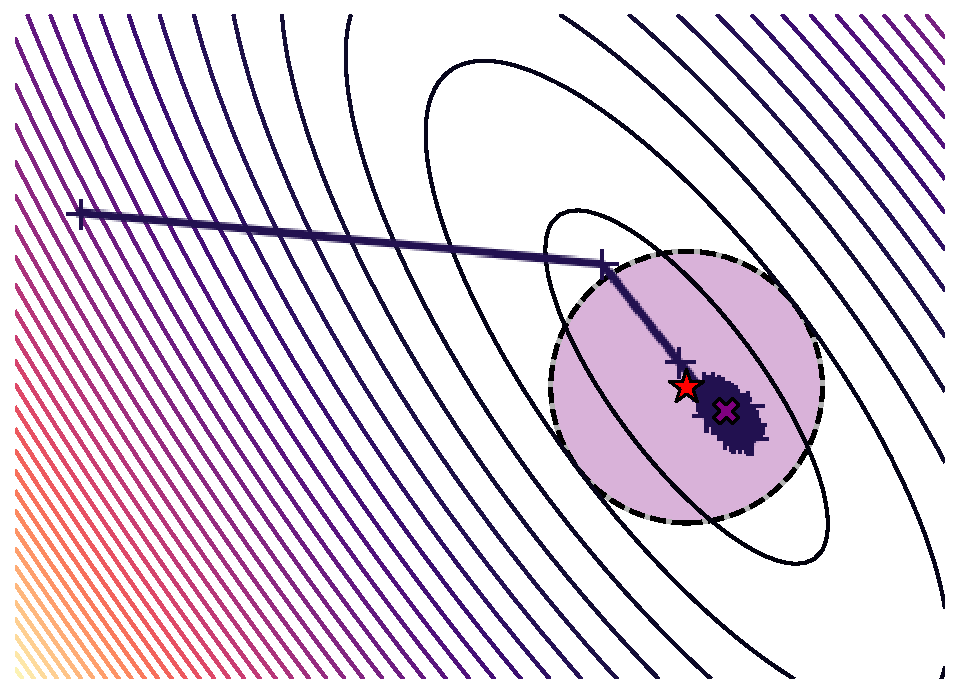
\includegraphics[width=0.3\linewidth]{images/plots/fedavg_True_10_t1000_s1.pdf}
  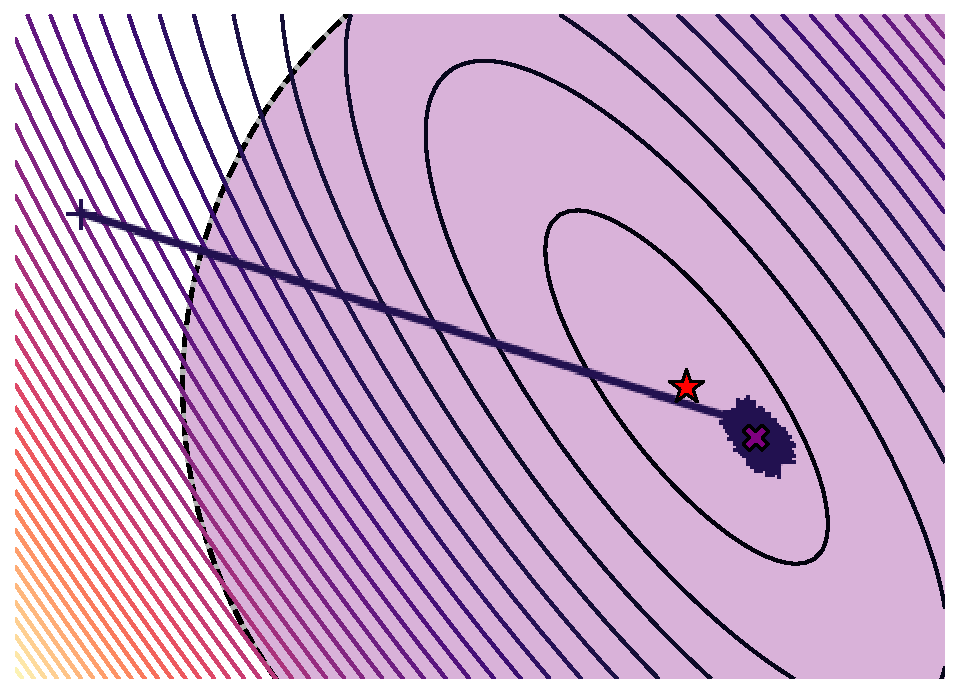
\includegraphics[width=0.3\linewidth]{images/plots/fedavg_True_50_t1000_s1.pdf}

\vspace{-3em}

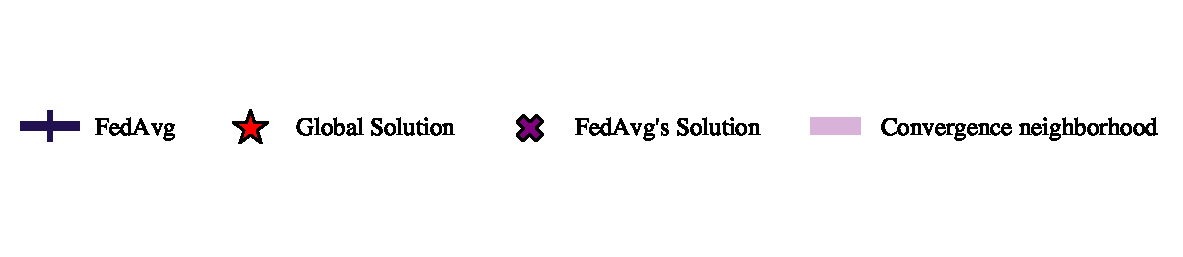
\includegraphics[width=0.8\linewidth]{images/legend_fedavg.pdf}    
    
  \end{center}

  \vspace{-3em}

  \pause
  \begin{tikzpicture}[remember picture, overlay]
        \node[widepinkblock]
        at (current page.center) {
        \huge
        Short answer: it also converges!
        };
    \end{tikzpicture}
\end{frame}


% \begin{frame}[t]{Federated Averaging\footfullcite{mcmahan2017communicationoral} ~~~ \raisebox{0.2em}{\textcolor{black}{\normalsize $x^\star \in \arg\min_{x \in \mathbb{R}^d} 
%     \frac{1}{N} \sum_{c=1}^N \mathbb{E}_Z[ F_c(x; Z) ]$}} ~~}  
    
%     \vspace{1em}

%   \begin{minipage}{0.5\linewidth}

%   \footnotesize
%   At each global iteration

%     \begin{itemize}[leftmargin=*,itemsep=0em]
%   \footnotesize
%     \item For $c=1$ à $N$ in parallel

% \vspace{-0.2em}
    
    
% \begin{itemize}[leftmargin=*,itemsep=0em]
% \item Receive $x^{(t)}$, set $x^{(t,0)}_c = x^{(t)}$
    
%         \item For $h=0$ to $H-1$
%     \end{itemize}

% \vspace{-0.6em}
% \begin{center}
%             \hspace{-1em}$x^{(t,h+1)}_c = x^{(t,h)}_c - \gamma \nabla F_c( x^{(t,h)}_c ; Z_c^{(t,h+1)})$
%         \end{center}
      
%   \item Aggregate local models 
        
        
% \vspace{-0.6em}
% \begin{center}
%             \hspace{-1em}$x^{(t+1)} = \frac{1}{N} \sum_{c=1}^N x_c^{(t,H)}$
%         \end{center}
      
%     \end{itemize}
      
%   \end{minipage}~%
%   \begin{minipage}{0.48\linewidth}
%     \pause
%     \begin{center}
%       \small
%     With deterministic gradients:
%     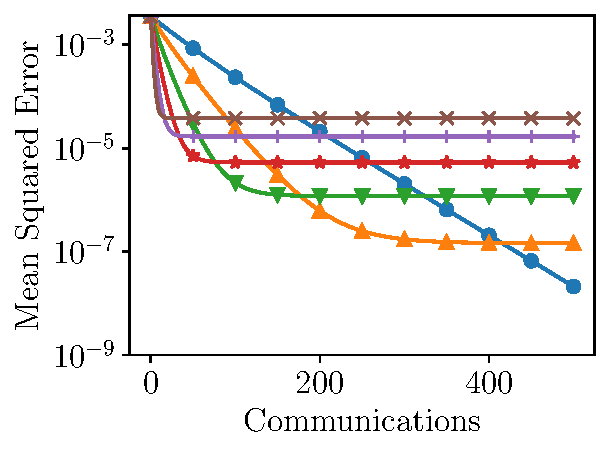
\includegraphics[width=0.75\linewidth]{images/local_training_heterogeneous.pdf}%
%     \raisebox{2.5em}{ 
\includegraphics[width=0.25\linewidth]{images/legend.pdf} }
%   \end{center}
  
%   %   \vspace{-0.5em}

%   % ~~~~Plus d'itérations locales

%   %   \vspace{0.5em}
    
%   %   ~~~~~{\large \textcolor{green} \cmark}\, convergence plus rapide
    
%   %   ~~~~~{\large \textcolor{red} \xmark}~ biais plus grand

%   \end{minipage}

%   \vspace{1.5em}


% \end{frame}

% \begin{frame}{Classical analyses of this algorithm\\[-0.5em]
%     \small (For $L$-smooth, $\mu$-strongly convex functions)}

%   Choose your favorite heterogeneity measure
%   \begin{itemize}
%   \item first-order\footfullcite{lian2017can}: $\zeta = \frac{1}{N} \sum_{c=1}^N \big\| \nabla f_c(x^{\star}) - \nabla f(x^{\star}) \big\|^2$
%   \item second-order\footfullcite{khaled2022faster}: $\zeta = \frac{1}{N} \sum_{c=1}^N \big\| \nabla_c^2 f(x^{\star}) - \nabla^2 f(x^{\star}) \big\|^2$
%   \item average drift\footfullcite{wang2024Unreasonable}: $\zeta = \big\| \frac{1}{NH} \sum_{c=1}^N \sum_{h=0}^{H-1} \nabla f(x_c^{(h)}) - \nabla f(x^{\star}) \big\|^2$
%   \end{itemize}

%   \vspace{0.5em}

%   \pause

%   Show \textcolor{purple}{\bfseries convergence to a neighborhood} of $x^\star$
%   \begin{align*}
%     \| x^{(T)} - x^\star \|^2 \lesssim (1 - \gamma \mu)^{HT} \| x^{(0)} - x^\star \|^2
%     + \textcolor{purple}{\boldsymbol{\chi(\gamma, H, \zeta)}} ~~~~~\text{\small (for some function $\chi$)}
%   \end{align*}

%   \vspace{1em}

  
% \end{frame}


% \begin{frame}[t]

%   \vspace{1em} 
%   \begin{center}
    
%   \resizebox{0.9\linewidth}{!}{
%   \begin{tikzpicture}
%     \draw [-to,very thick](0,0) -- (12.5,0);
%     \node at (1.5,0.2) {$H=2$};
%     \node at (6,0.2) {$H=10$};
%     \node at (10.5,0.2) {$H=50$};
%   \end{tikzpicture}
% }
% \vspace{-0.5em}

% \only<1>{
%   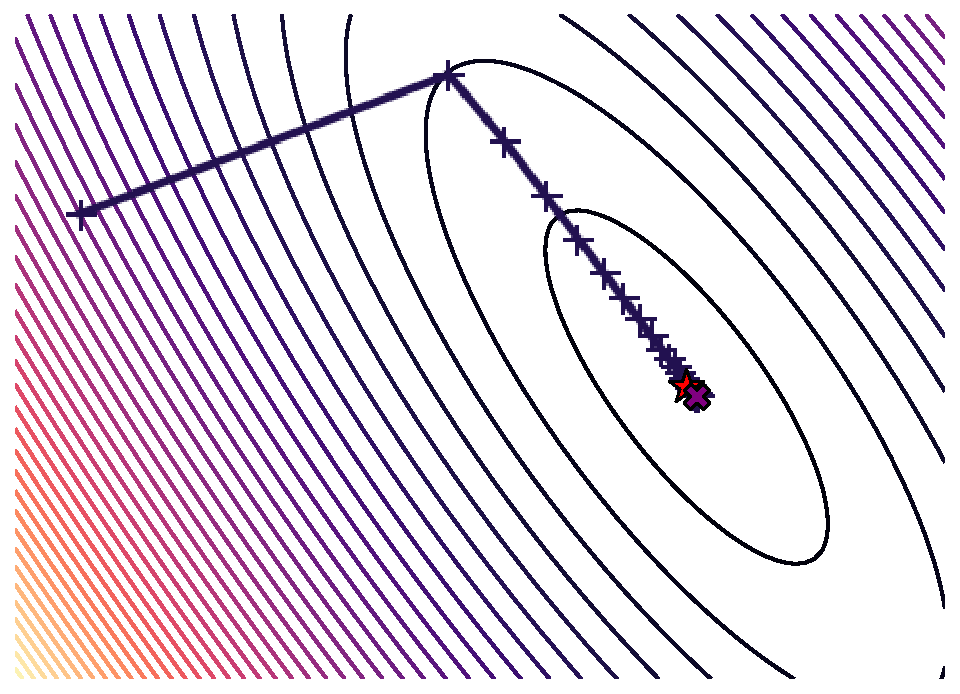
\includegraphics[width=0.3\linewidth]{images/plots/fedavg_False_2_t1000_s0.pdf}
%   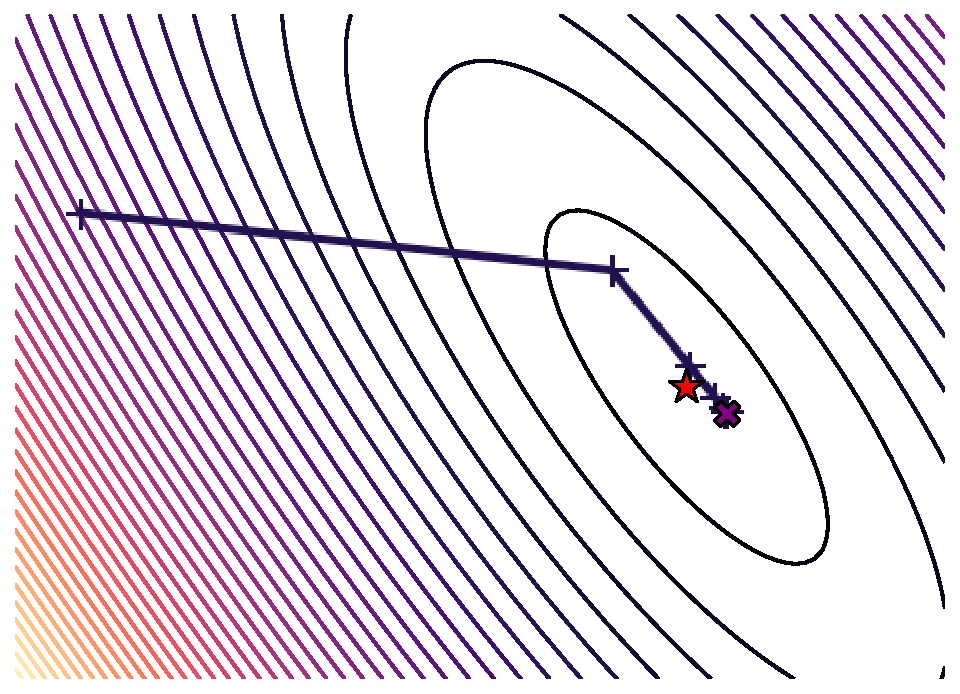
\includegraphics[width=0.3\linewidth]{images/plots/fedavg_False_10_t1000_s0.pdf}
%   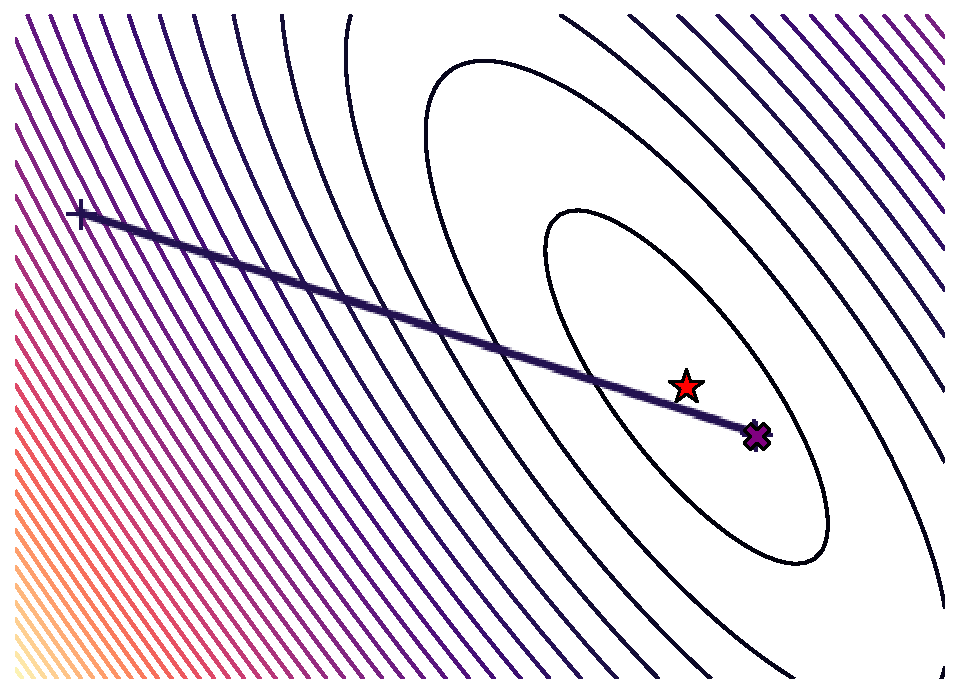
\includegraphics[width=0.3\linewidth]{images/plots/fedavg_False_50_t1000_s0.pdf}
% }%
% \only<2,3>{
%   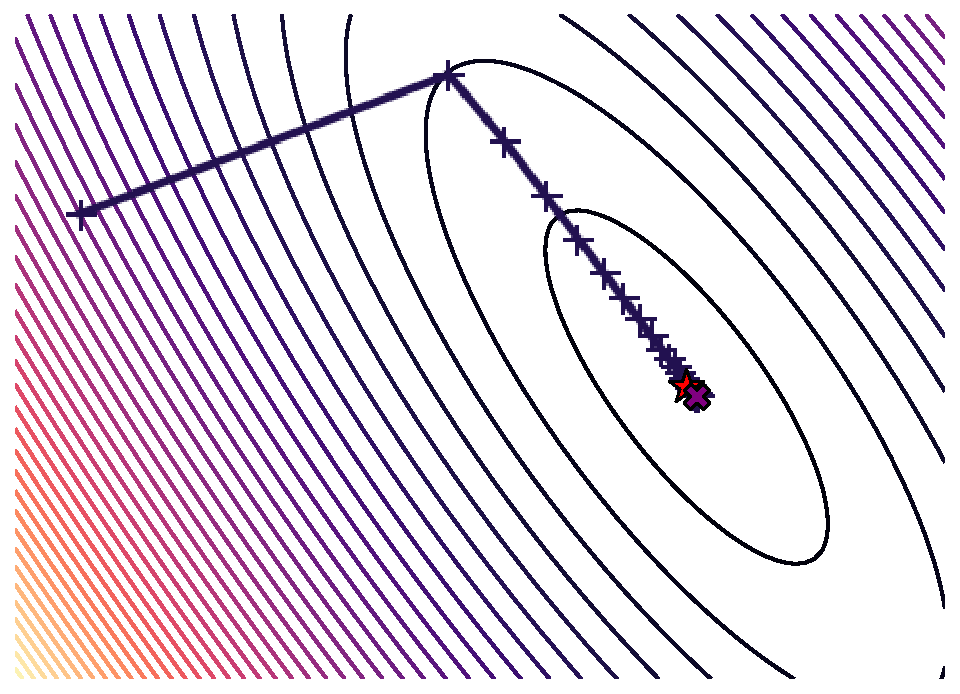
\includegraphics[width=0.3\linewidth]{images/plots/fedavg_True_2_t1000_s0.pdf}
%   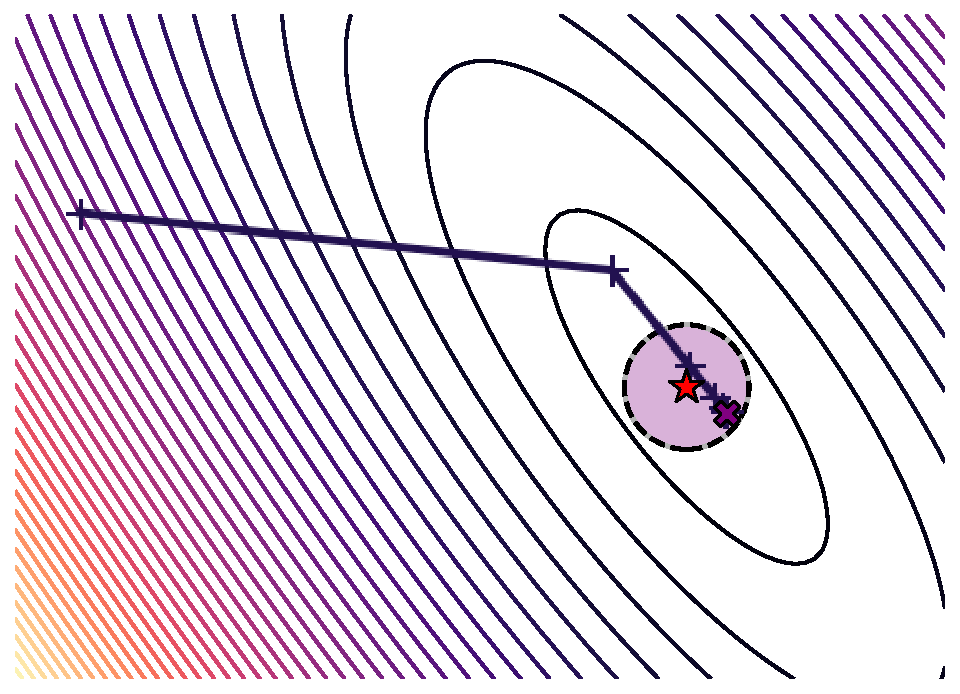
\includegraphics[width=0.3\linewidth]{images/plots/fedavg_True_10_t1000_s0.pdf}
%   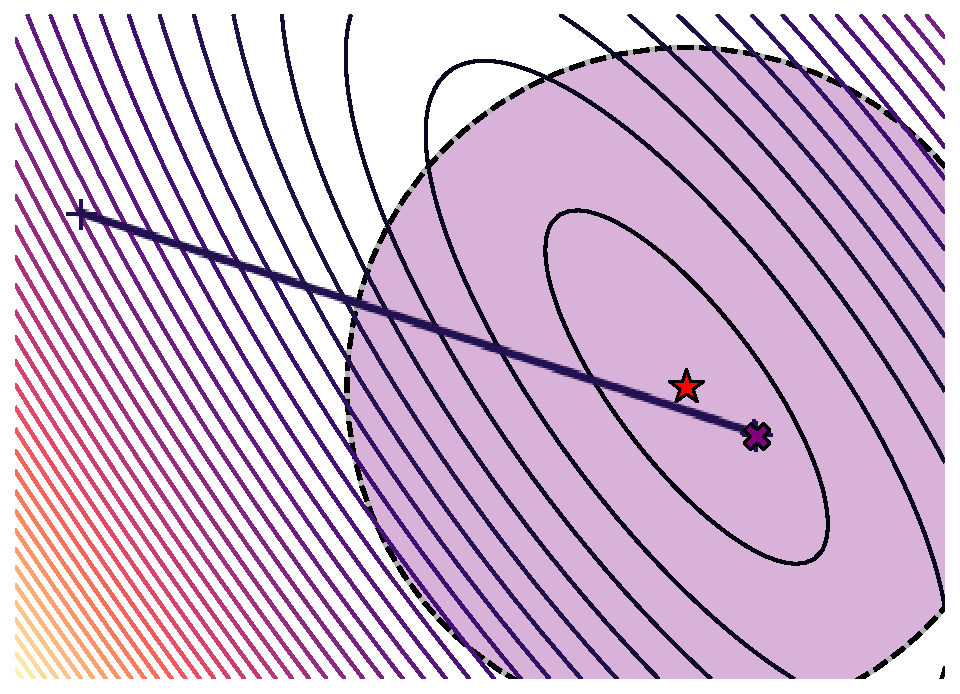
\includegraphics[width=0.3\linewidth]{images/plots/fedavg_True_50_t1000_s0.pdf}
% }%
% \only<4>{
%   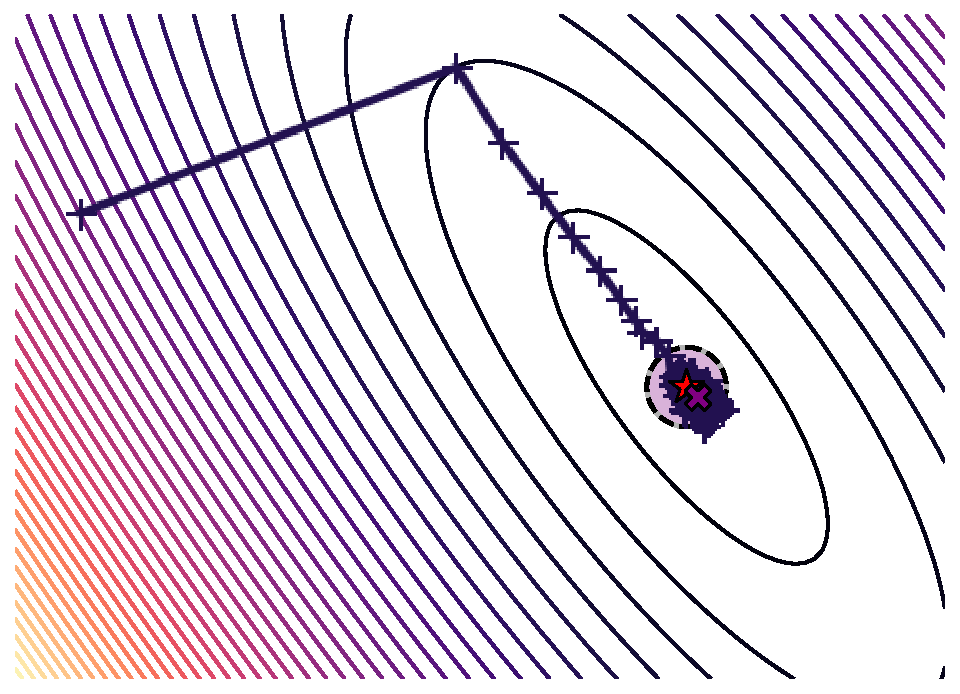
\includegraphics[width=0.3\linewidth]{images/plots/fedavg_True_2_t1000_s1.pdf}
%   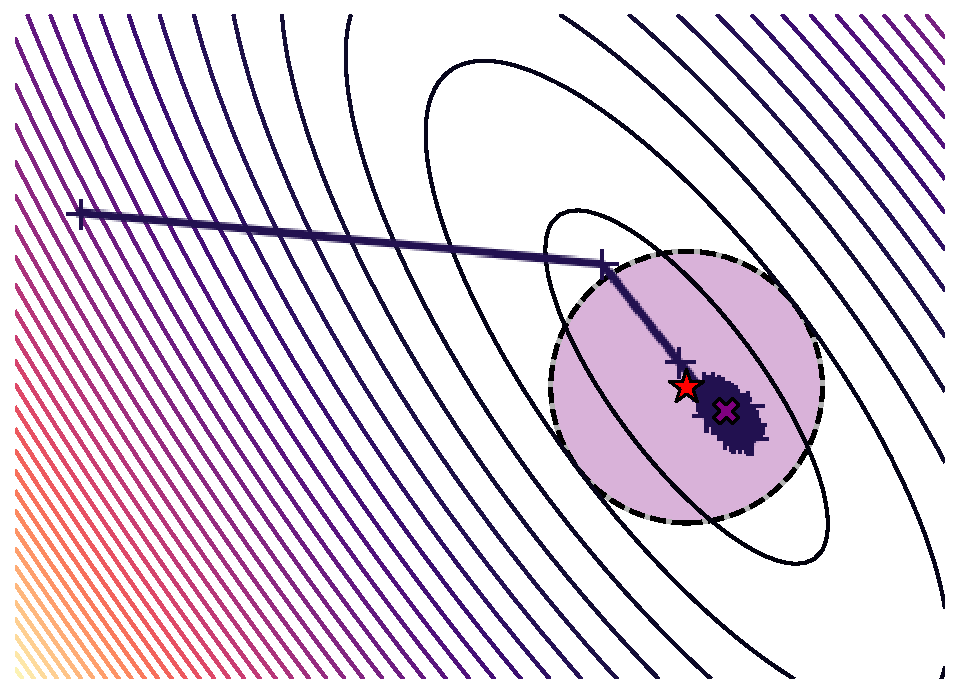
\includegraphics[width=0.3\linewidth]{images/plots/fedavg_True_10_t1000_s1.pdf}
%   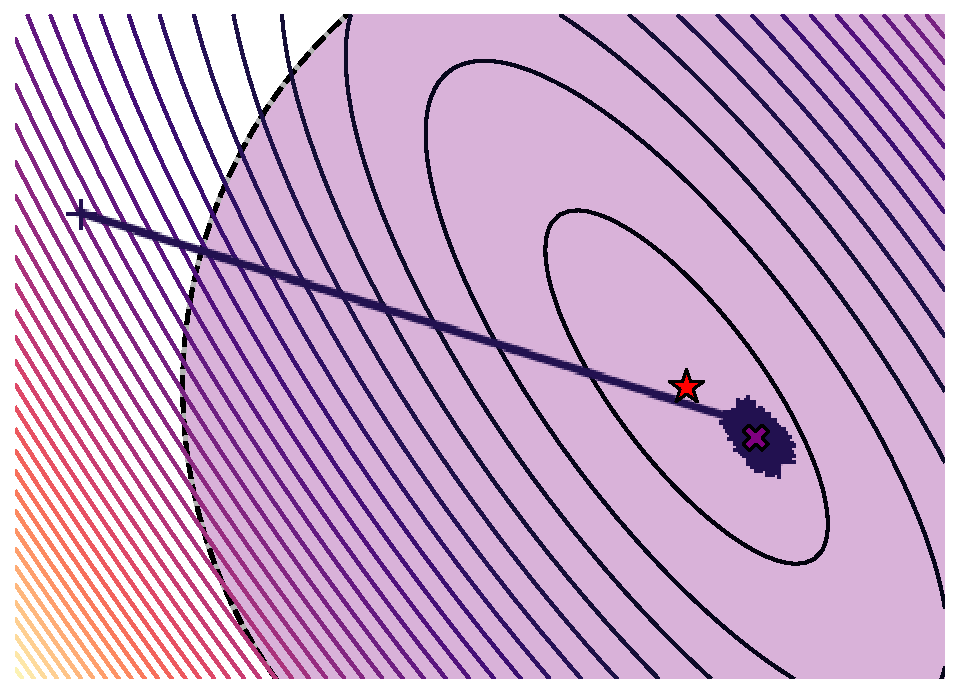
\includegraphics[width=0.3\linewidth]{images/plots/fedavg_True_50_t1000_s1.pdf}
% }

% \vspace{-3em}

% 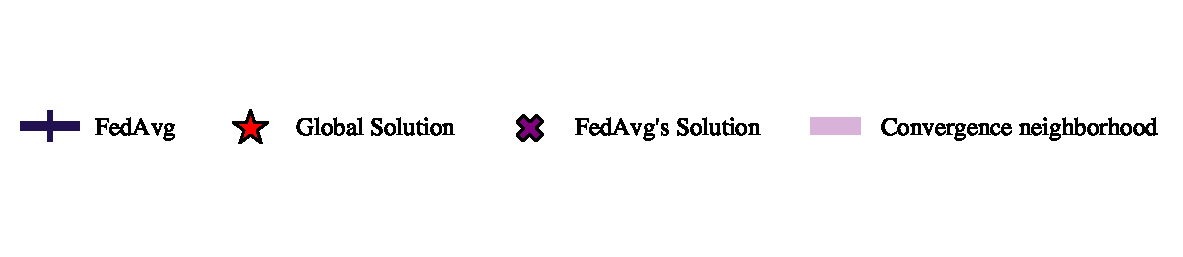
\includegraphics[width=0.8\linewidth]{images/legend_fedavg.pdf}    
    
%   \end{center}

%   \vspace{-3em}

%   \begin{center}
%     When the number of local iterations increases, bias incrases

%     \pause
    
%     ... but the bound is oblivious to problem's geometry
    

%   \pause
  
%   \textcolor{purple}{\bfseries Remark:} It seems that iterates converge in some way?
%   \end{center}
  
% \end{frame}




\begin{frame}[t]{FedAvg (with stochastic gradients) converges!\footfullcite{mangold2025refined}\\[-0.5em]
      \small (For thrice derivable, $L$-smooth, $\mu$-strongly convex functions)}
    
\begin{itemize}[leftmargin=*]
    \item FedAvg converges to a stationary distribution $\pi^{(\gamma, H)}$
    \only<1>{
    \begin{itemize}
        \item denoting $x^{(t)} \sim \psi_{x^{(t)}}$, we have
    \begin{align*}
        \mathcal{W}_2(\psi_{x^{(t)}}; \pi^{(\gamma, H)})
        \le
        (1 - \gamma \mu)^{H t} \mathcal{W}_2(\psi_{x^{(0)}}; \pi^{(\gamma, H)})
    \end{align*}
    \item where $\mathcal{W}_2$ is the second order Wasserstein distance
    \end{itemize}
    }

\pause

    \item FedAvg's iterates covariance is
    \only<2,3>{
    \begin{align*}
    \int (x - x^\star)(x - x^\star)^\top \pi^{(\gamma, H)}(\mathrm{d} x)
    &  =
    \tikz[remember picture,baseline=(variance.base)] \node[pinkblock] (variance) at (0,0) {
    \textnormal{$\displaystyle \frac{\gamma}{N} \boldsymbol{A} C(x^\star) $}}; + O(\gamma^{3/2} H)
    \end{align*}
    }

\only<3>{
\begin{tikzpicture}[overlay,remember picture]
    \node[pinkblock] (variancelegend) at (5,4) {\shortstack{\underline{Linear speed-up !} \\[0.5em]
    variance decreases in $1/N$ \\
    variance scales in $\gamma$
    }};
    \draw[color=amethyst] (variance) -- (variancelegend);
\end{tikzpicture}

\vspace{-4em}
}
\pause

\pause


    \item We can now give an \textcolor{purple}{\bfseries exact expansion of the bias}
    \only<4,5>{
    \begin{align*}
    \int x \pi^{(\gamma, H)}(\mathrm{d} x)
    &  = x^\star +
    \tikz[remember picture,baseline=(heterbias.base)] \node[blueblock] (heterbias) at (0,0) {
    \textnormal{$\displaystyle \frac{\gamma (H-1)}{2N}
    \sum_{c=1}^N \nabla^2 f(x^\star)^{-1}
    \big( \nabla^2 f_c(x^\star) - \nabla^2 f(x^\star) \big)
    \nabla f_c(x^\star)$}
    };
    \\ 
    &  \qquad
    -  \tikz[remember picture,baseline=(stobias.base)] \node[pinkblock] (stobias) at (0,0) {
    \textnormal{$\displaystyle
    \frac{\gamma}{2 N} \nabla^2 f(x^\star)^{-1}
    \nabla^3 f(x^\star) \boldsymbol{A} C(x^\star)
    $}};
    + O(\gamma^{3/2} H)
    \end{align*}
    }
\pause

\only<4,5>{
\begin{tikzpicture}[overlay,remember picture]
    \node[blueblock] (heterbiaslegend) at (3,6) {\shortstack{\underline{Heterogeneity bias} \\[0.5em]
     vanishes when $\nabla^2 f_c(x^\star) = \nabla^2 f(x^\star)$ \\
    \quad or when $\nabla f_c(x^\star) = \nabla f(x^\star)$
    }};
    \draw[color=amethyst] (heterbias) -- (heterbiaslegend);
    
    \node[pinkblock] (stobiaslegend) at (10.5,6) {\shortstack{\underline{Stochasticity bias} \\[0.5em]
    $\boldsymbol{A} = (I \otimes \nabla^2 f(x^\star) + \nabla^2 f(x^\star) \otimes I)^{-1} $ \\
    $C(x^\star)$ is $\nabla F^Z$'s covariance at $x^\star$
    }};
    \draw[color=amaranth] (stobias) -- (stobiaslegend);
\end{tikzpicture}

\vspace{-4em}
}

\end{itemize}

\vspace{4em}

\end{frame}


\begin{frame}{Correcting the Bias\\[-0.2em]
\large Novel Algorithm: Federated Richardson-Romberg Extrapolation}
    Run FedAvg twice:
    \begin{itemize}
        \item with step size $\gamma$: global iterates $x_{\gamma}^{(t)}$
        \item with step size $2 \gamma$: global iterates $x_{2 \gamma}^{(t)}$
    \end{itemize}

    We can combine the iterates
    \begin{align*}
        \chi_{\text{RR}}^{(t)}
        =
        2 x_{\gamma}^{(t)}
        - x_{2 \gamma}^{(t)}
    \end{align*}

    \pause
    \begin{tikzpicture}[remember picture, overlay]
        \node[widepinkblock]
        at (current page.center) {
        \shortstack{\large
        Theorem:
        $\mathbb{E} [ \chi_{\text{RR}}^{(t)} ] = x_\star + O(\gamma^2 H^2 + \gamma^{3/2} H)$
        \\[1em]
        \large 
        $\rightarrow$ bias is effectively reduced!!
        }};
    \end{tikzpicture}
\end{frame}

\begin{frame}{Numerical Illustration: FedAvg}
\begin{figure}[t]
    \centering
     \begin{subfigure}[b]{0.45\linewidth}
         \centering
         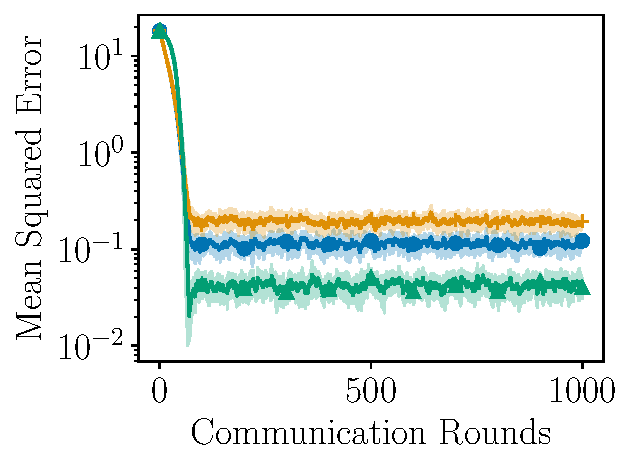
\includegraphics[width=\textwidth]{images/plots/heterogeneous_iterates_10.pdf}
         \caption{$H=10$}
     \end{subfigure}
     \begin{subfigure}[b]{0.45\linewidth}
         \centering
         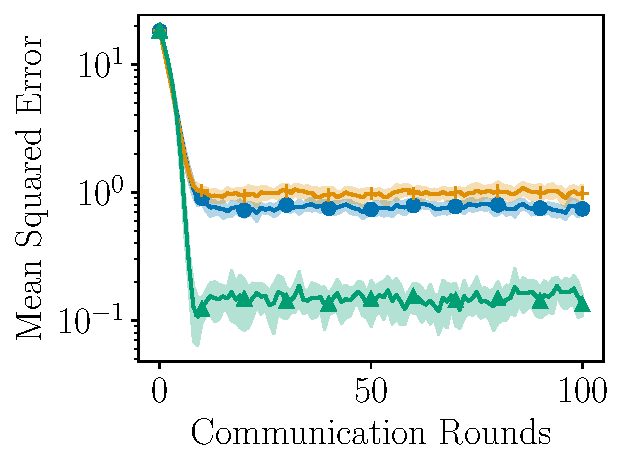
\includegraphics[width=\textwidth]{images/plots/heterogeneous_iterates_100.pdf}
         \caption{$H=100$}
     \end{subfigure}
     \end{figure}
     \vspace{-1em}
     \begin{center}
     Blue: FedAvg,~
     Orange: Scaffold,~
     Green: Federated Richardson-Romberg
     \end{center}
\end{frame}


\begin{frame}
  \begin{center}
    \huge \textcolor{purple}{
      II. Correcting heterogeneity: Scaffold
      }
  \end{center}
\end{frame}


\begin{frame}[t]{Scaffold\footfullcite{karimireddy2020scaffoldshort} ~~~ \raisebox{0.2em}{\textcolor{black}{\normalsize $x^\star \in \arg\min_{x \in \mathbb{R}^d} 
        \frac{1}{N} \sum_{c=1}^N \mathbb{E}_Z[ F_c(x; Z) ]$}} ~~\\[-0.5em]
  \normalsize ($^*$without global step size) \qquad \qquad \qquad \qquad \qquad \qquad \qquad \qquad \qquad \qquad}  
    
%    \vspace{-1em}

  \begin{minipage}{0.5\linewidth}

  \footnotesize
  At each global iteration

    \begin{itemize}[leftmargin=*,itemsep=0em]
  \footnotesize
    \item For $c=1$ to $N$ in parallel

\vspace{-0.2em}
    
    
\begin{itemize}[leftmargin=*,itemsep=0em]
\item Receive $x^{(t)}$, set $x^{(t,0)}_c = x^{(t)}$
    
        \item For $h=0$ to $H-1$
    \end{itemize}

\vspace{-0.6em}
\begin{center}
            \hspace{-1em}$x^{(t,h+1)}_c = x^{(t,h)}_c - \gamma \big( \nabla F_c( x^{(t,h)}_c ; Z_c^{(t,h+1)}) + \textcolor{purple}{\boldsymbol{\xi_c^{(t)}}} \big)$
        \end{center}
      
  \item Aggregate models, update control variates
        
        
\vspace{-0.6em}
\begin{center}
            \hspace{-1em}$x^{(t+1)} = \frac{1}{N} \sum_{c=1}^N x_c^{(t,H)}$
          \end{center}
\begin{center}
            \hspace{-1em}$\textcolor{purple}{\boldsymbol{\xi_c^{(t+1)} = \xi_c^{(t)} + \frac{1}{\gamma H} (x_c^{t,H} - x^{(t+1)} )}}$
          \end{center}

          
      
    \end{itemize}
      
  \end{minipage}~~~~~~%
  \begin{minipage}{0.48\linewidth}
  \pause
       \begin{center}
    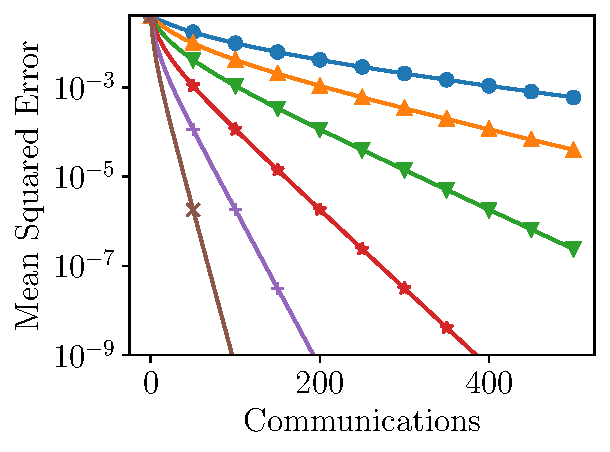
\includegraphics[width=0.75\linewidth]{images/local_training_homogeneous.pdf}%
    \raisebox{2.5em}{ 
\includegraphics[width=0.25\linewidth]{images/legend.pdf} }
  \end{center}
  
    \vspace{-0.5em}

  $\rightarrow$ No more heterogeneity bias!

  \end{minipage}

  \vspace{1.5em}


\end{frame}




\begin{frame}[t]{Scaffold also converges !\footfullcite{mangold2025scaffold}\\[-0.5em]
  \small (For $L$-smooth, $\mu$-strongly convex functions with $\nabla^3 f(x)$ bounded by $Q$)}


\begin{itemize}[leftmargin=*]
    \item Scaffold converges if $\gamma H L \le 1$, towards a distribution $\pi^{(\gamma, H)}$
    \only<1>{
    \begin{itemize}
        \item denoting $(x^{(t)}, \xi_{1:N}^{(t)}) \sim \psi_{(x^{(t)}, \xi_{1:N}^{(t)})}$, we have
    \begin{align*}
        \mathcal{W}_2(\psi_{(x^{(t)}, \xi_{1:N}^{(t)})}; \pi^{(\gamma, H)})
        \le
        (1 - \gamma \mu)^{H t} \mathcal{W}_2(\psi_{(x^{(t)}, \xi_{1:N}^{(t)})}; \pi^{(\gamma, H)})
    \end{align*}
    \item where $\mathcal{W}_2$ is the second order Wasserstein distance
    \end{itemize}
    }

    \pause
    
  \item Scaffold's variance is close to FedAvg's variance
    \only<2,3>{
      \begin{align*}
        \int (x - x^\star)(x - x^\star)^\top \pi^{(\gamma, H)}(\mathrm{d} x, \rmd \Xi)
        &  =
          \tikz[remember picture,baseline=(variance.base)] \node[pinkblock] (variance) at (0,0) {
          \textnormal{$\displaystyle \frac{\gamma}{N} \boldsymbol{A} C(x^\star) $}}; + O(\gamma^{3/2})
      \end{align*}
    }
    \pause
    
    \only<3>{
      \begin{tikzpicture}[overlay,remember picture]
        \node[pinkblock] (variancelegend) at (5,4) {\shortstack{\underline{Linear speed-up !} \\[0.5em]
            variance decreases in $1/N$ \\
            variance scales in $\gamma$
          }};
        \draw[color=amethyst] (variance) -- (variancelegend);
      \end{tikzpicture}
      
      \vspace{-4em}
    }

    \pause

  \item Scaffold \textbf{\textcolor{purple}{removes heterogeneity bias}}
    \only<4,5>{
      \begin{align*}
        \int x \pi^{(\gamma, H)}(\mathrm{d} x, \rmd \Xi)
        &  = x^\star
          -  \tikz[remember picture,baseline=(stobias.base)] \node[pinkblock] (stobias) at (0,0) {
          \textnormal{$\displaystyle
          \frac{\gamma}{2 N} \nabla^2 f(x^\star)^{-1}
          \nabla^3 f(x^\star) \boldsymbol{A} C(x^\star)
          $}};
          + O(\gamma^{3/2})
      \end{align*}
    }

    \only<5>{
      \begin{tikzpicture}[overlay,remember picture]    
        \node[pinkblock] (stobiaslegend) at (10.5,4) {\shortstack{\underline{Stochasticity bias remains} \\[0.5em]
            $\boldsymbol{A} = (I \otimes \nabla^2 f(x^\star) + \nabla^2 f(x^\star) \otimes I)^{-1} $ \\
            $C(x^\star)$ is $\nabla F^Z$'s covariance at $x^\star$
          }};
        \draw[color=amaranth] (stobias) -- (stobiaslegend);
      \end{tikzpicture}
      
      \vspace{-0.5em}
    }%
      \textbf{\textcolor{purple}{$\Rightarrow$ but it is still biased}}


\pause

\end{itemize}

\end{frame}
\begin{frame}[t]

  \vspace{1em}
  
  \begin{center}
    
  \resizebox{0.9\linewidth}{!}{
  \begin{tikzpicture}
    \draw [-to,very thick](0,0) -- (12.5,0);
    \node at (1.5,0.2) {$H=10$};
    \node at (6,0.2) {$H=20$};
    \node at (10.5,0.2) {$H=50$};
  \end{tikzpicture}
}
\vspace{-0.5em}

\only<1>{
  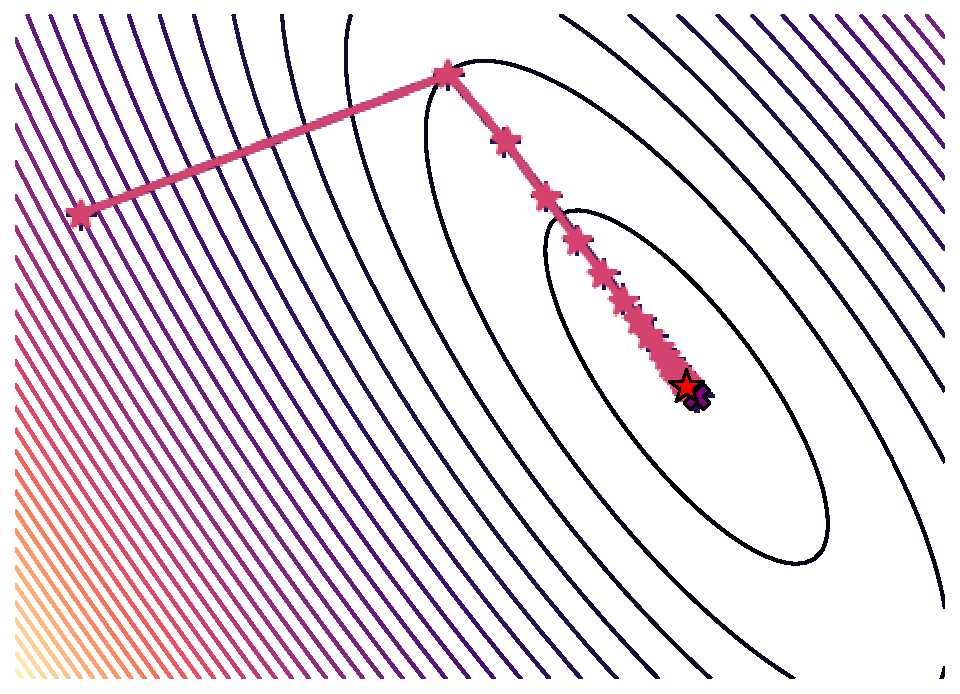
\includegraphics[width=0.3\linewidth]{images/plots/fedavg_scaffold_True_2_t1000_s0.pdf}
  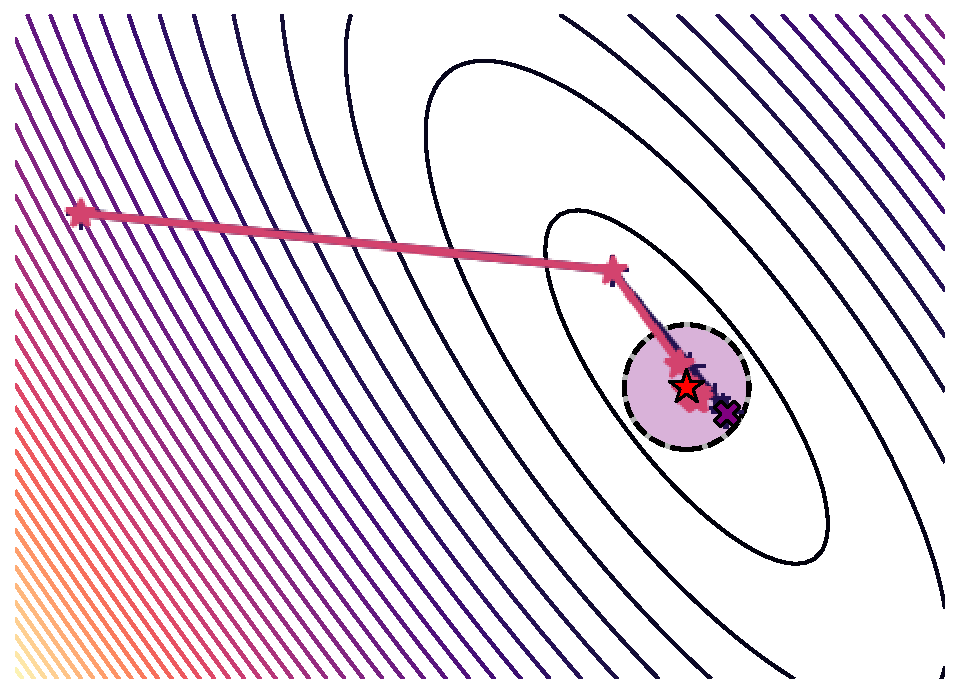
\includegraphics[width=0.3\linewidth]{images/plots/fedavg_scaffold_True_10_t1000_s0.pdf}
  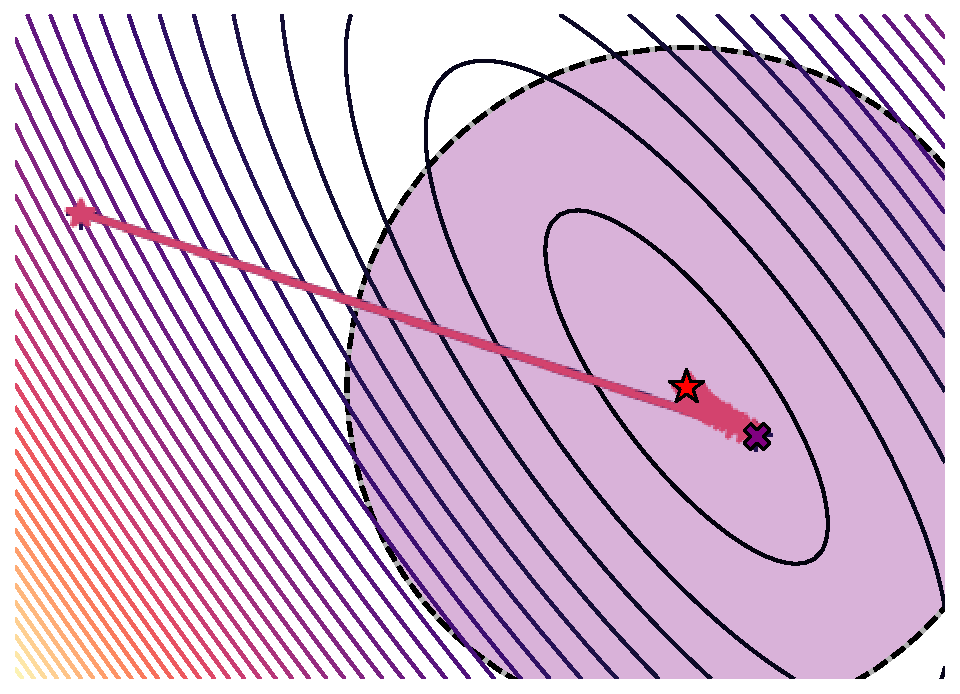
\includegraphics[width=0.3\linewidth]{images/plots/fedavg_scaffold_True_50_t1000_s0.pdf}
}%
\only<2>{
  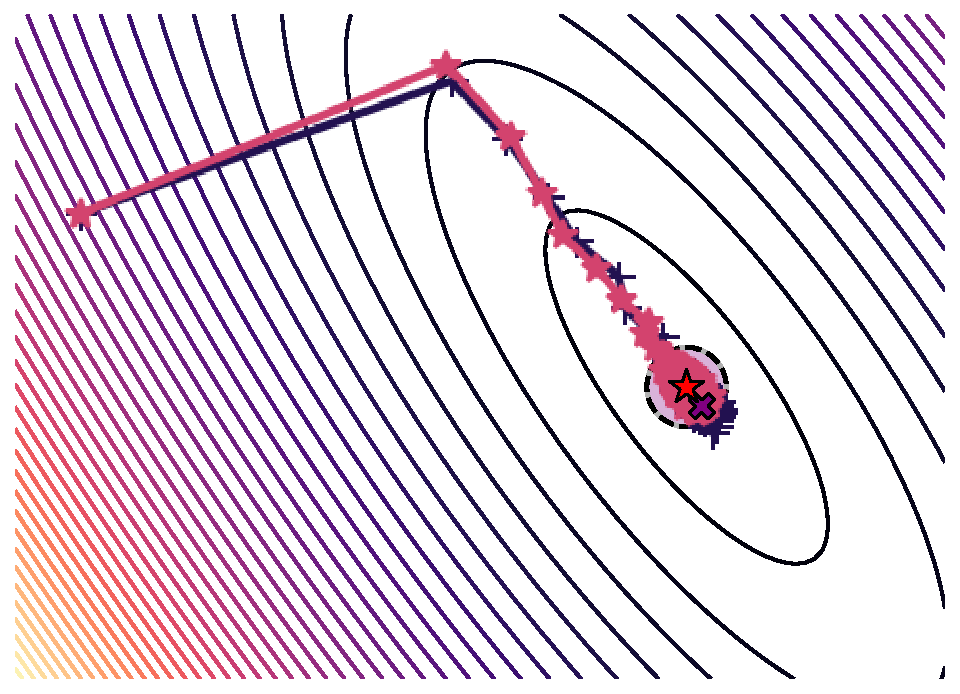
\includegraphics[width=0.3\linewidth]{images/plots/fedavg_scaffold_True_2_t1000_s1.pdf}
  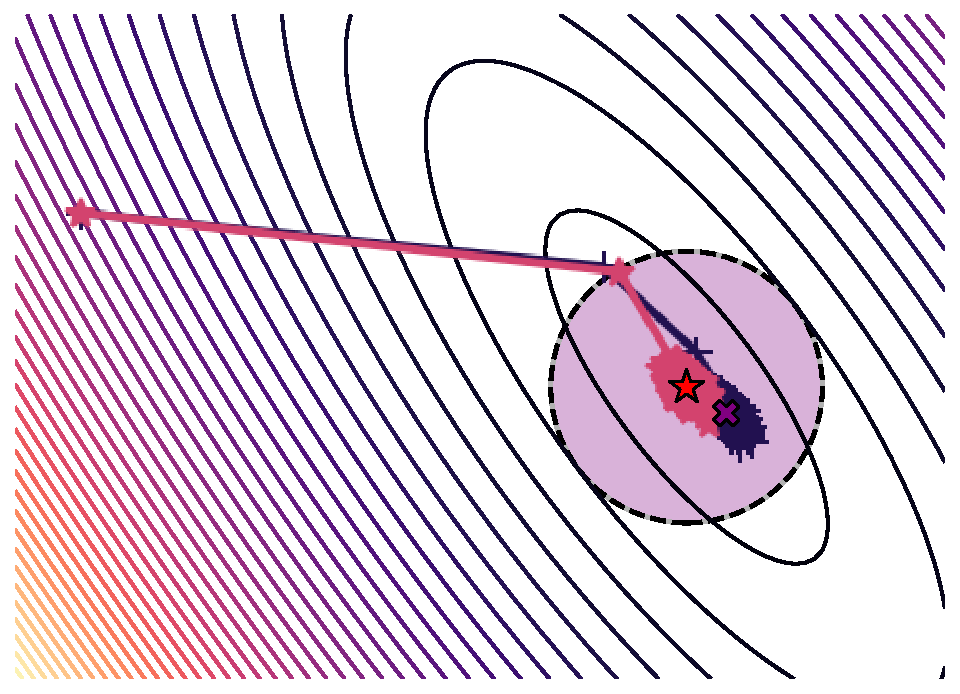
\includegraphics[width=0.3\linewidth]{images/plots/fedavg_scaffold_True_10_t1000_s1.pdf}
  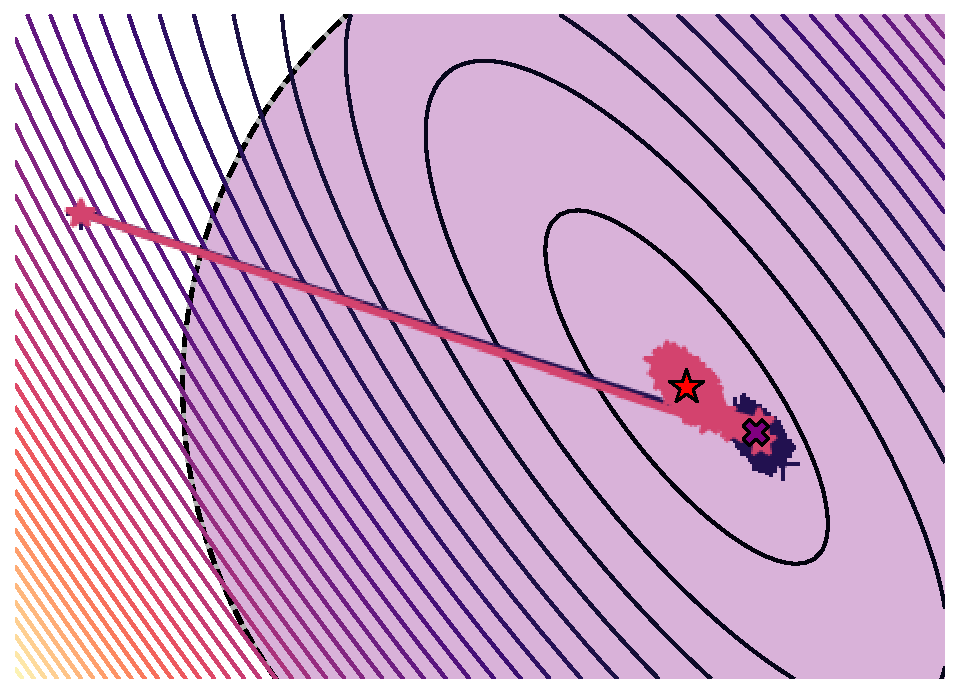
\includegraphics[width=0.3\linewidth]{images/plots/fedavg_scaffold_True_50_t1000_s1.pdf}
}


\vspace{-3em}

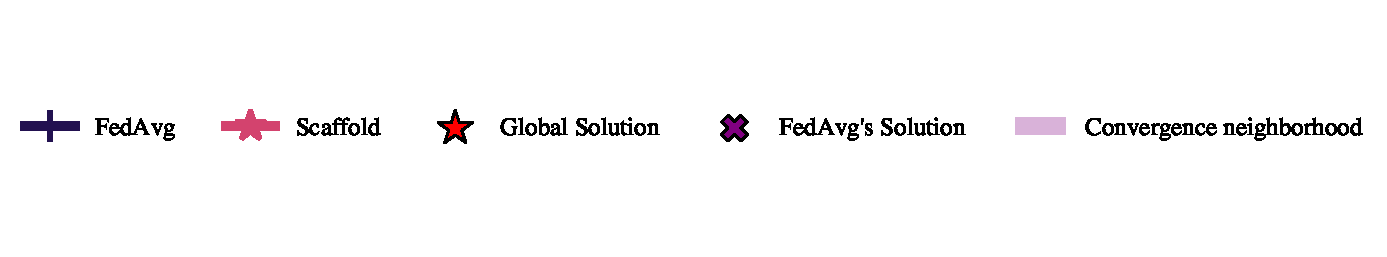
\includegraphics[width=\linewidth]{images/legend_fedavg_scaffold.pdf}    

\end{center}

  \vspace{-3em}
  \begin{center}
    Scaffold converges to the right point


    ... and its variance is similar to FedAvg!
  \end{center}


\end{frame}

\begin{frame}{Bounding the Covariance}
  Define covariance matrices
\begin{align*}
% \textbf{Limit point}\qquad~ \statdistlim{\step,\nlupdates} & \eqdef {\int} \varparam \statdist{\step, \nlupdates}(\rmd \varparam, \rmd \Xi)
% \\[0.5em]
%   \textbf{Covariance}\qquad\quad~ 
  \covparam &
\eqdef\! \int \big(\param - \paramlim\big)^{\otimes 2} \statdist{\step, \nlupdates}(\rmd \param, \rmd \Xi) 
  \\
  \covcvar{c,c'} 
& \eqdef 
\int \big( \xi_{c}{} \!- \xi_c^{\star} \big)
\big( \xi_{c'}{} \!- \xi_c^{\star} \big)^\top \statdist{\step, \nlupdates}( \rmd \param, \rmd \Xi )
\\
\covparamcvar{c}
& \eqdef{}\!
\int 
\big( \param - \paramlim \big) \big( \xi_{c}{} \!- \xi_{c}^{\star} \big)^\top 
\statdist{\step, \nlupdates}( \rmd \param, \rmd \Xi )
\end{align*}

\end{frame}

\begin{frame}{Expansion of Covariance}
  \vspace{-1em}
  
\begin{align*}
\covparam
& =
\tfrac{\step}{\nagent} \boldsymbol{A} \covfunc(\paramlim)
+ O(\step^2 H + \step^{3/2})
\\[0.5em]
\covparamcvar{c}
& =
  \tfrac{\step}{\nagent} \boldsymbol{A} \covfunc(\paramlim) (\hnf{c}{\paramlim} - \hf{\paramlim})
 + \tfrac{\step}{\nagent}
\left( \loccovfunc{c}(\paramlim) - \covfunc(\paramlim)  \right)
+ O(\step^2 H + \step^{3/2})
\\[0.5em]
\covcvar{c,c} & =
( 1 - \tfrac{2}{\nagent} )
\tfrac{1}{H} \loccovfunc{c}(\paramlim)
+ \tfrac{1}{\nagent H} \covfunc(\paramlim)
+ O(\step)
\\[0.5em]
\covcvar{c,c'} & =
\tfrac{1}{\nagent H} ( \covfunc(\paramlim) 
- \loccovfunc{c}(\paramlim) 
- \loccovfunc{c'}(\paramlim))
+ O(\step)
\end{align*} 

\vspace{1em}
    
    \textbf{\textcolor{purple}{where}}
    \vspace{-1.5em}
        \begin{equation*}
        \begin{aligned}
        \boldsymbol{A} 
        &\eqdef (\Id \otimes \hf{\paramlim} + \hf{\paramlim} \otimes \Id)^{-1}
        \\
        \loccovfunc{c}(\paramlim) 
        \eqdef \mathbb{E} \Big[&  \big( \gnfs[c]{\paramlim}{Z_c} \!-\! \gnf[c]{\paramlim} \big)^{\otimes 2} \Big]
                         ~
                         \covfunc(\paramlim) \eqdef \frac{1}{\nagent} \sum_{c=1}^{\nagent}
          \loccovfunc{c}(\paramlim)
        \end{aligned}
      \end{equation*}
  
\end{frame}



\begin{frame}{New Convergence Rate for Scaffold\\[-0.5em]
    \small (For $L$-smooth, $\mu$-strongly convex functions with $\nabla^3 f(x)$ bounded by $Q$)}
\begin{align*}
\mathbb{E}\left[ \| x^{(T)} - x^\star \|^2 \right] 
& \lesssim{} \left( 1 - \frac{\gamma \mu}{4} \right)^{HT}
\left\{ 
\| x^{(0)} - x^\star \|^2
+
2\gamma^2 H^2 \zeta^2
+
\frac{ \sigma_\star^2 }{L\mu}
\right\}
\\ &  \quad\quad\quad\quad\quad\quad\quad
+ 
\frac{\gamma }{\textcolor{purple}{\boldsymbol{N}} \mu} \sigma_\star^2 
+ \frac{ \gamma^{3/2} Q }{\mu^{5/2}} \sigma_\star^3
+ \frac{ \gamma^3 H Q^2}{\mu^3} \sigma_\star^4
\end{align*}


where
\begin{itemize}
\item \small
  $\sigma_\star^2 = \mathbb{E}[ \frac{1}{N} \sum_{c=1}^N \| \nabla F_c^Z(x^\star) - \nabla f_c(x^\star) \|^2$ is the variance at $x^\star$
\item \small
  $\zeta^2 = \frac{1}{N} \sum_{c=1}^N \| \nabla f_c^Z(x^\star) \|^2$ measures gradient heterogeneity
\end{itemize}



\end{frame}

\begin{frame}{Linear Speed-Up!}

  As long as $N$ is not too large, one can obtain $\mathbb{E}\left[ \| x^{(T)} - x^\star \|^2 \right] \le \epsilon^2 $ with
  \begin{align*}
    \# \text{grad per client}
    = \widetilde O\Big( \frac{\sigma_\star^2}{\textcolor{purple}{\boldsymbol{N}} \mu^2 \epsilon^2} 
    \log\left( 
    \frac{1}{\epsilon}
    \right) \Big)
  \end{align*}
  
\end{frame}

\begin{frame}{Conclusion}

  \begin{itemize}[itemsep=1em]
  \item FedAvg and Scaffold converge (even with stochastic gradients)
  \item This allows to derive new analyses for these problems,

    with exact first-order expression for bias
  \item And we proved that Scaffold has:
    \begin{itemize}
    \item variance similar to FedAvg's variance
    \item \textit{linear speed-up} in the number of clients!!
    \end{itemize}

  \item But: Scaffold is still biased
    
  \textbf{\textcolor{purple}{$\Rightarrow$ Need for algorithms tailored for FL \underline{and} stochasticity!}}
    
  \end{itemize}


\end{frame}



\begin{frame}
  \begin{center}
    \huge \textcolor{purple}{
      Thank you!
      }
    \end{center}

    Check the papers:
    \vspace{-1em}
    \begin{itemize}
    \item \small \fullcite{mangold2025refined}
    \item \small \fullcite{mangold2025scaffold}
    \end{itemize}

    Find this presentation on my website:
    \vspace{-1em}
    \begin{itemize}
    \item \textcolor{amaranth}{\url{https://pmangold.fr/research.php?page=talks}}
    \end{itemize}
    
\end{frame}


\end{document}
%%% Local Variables:
%%% mode: latex
%%% TeX-master: t
%%% End:
